\documentclass[letter]{beamer}
%removed: handout (ignores "animations")

\usepackage[utf8]{inputenc}
\usepackage{graphicx}
\usepackage{minted}

\usetheme{AnnArbor}
%\usetheme{CambridgeUS}
\usecolortheme{beaver}

\title[IIC2333] % (optional, only for long titles)
{06 - Capa Física y Capa de Enlace}
\subtitle{IIC2333 - Sistemas Operativos y Redes}
\author[C.Ruz] % (optional, for multiple authors)
{Cristian Ruz -- {\tt cruz@ing.puc.cl}\footnote{Material preparado con aporte del profesor Carlos Buil Aranda} }
\institute[PUC] % (optional)
{
  Departamento de Ciencia de la Computación\\
  Pontificia Universidad Católica de Chile
}
\date[2/2015] % (optional)
{Semestre 2-2015}
\subject{Informatik}

\AtBeginSection[]
{
  \begin{frame}
    \frametitle{Contenidos}
    \tableofcontents[currentsection]
  \end{frame}
}

\begin{document}

%---------------------------------------------------------------------
\frame{\titlepage}

%---------------------------------------------------------------------
\begin{frame}
\frametitle{Contenidos}
%\tableofcontents[currentsection]
\tableofcontents
\end{frame}


%---------------------------------------------------------------------
\section{Señales y Medios de Transmisión}

\subsection{Transmisión de señales}

\begin{frame}
  \frametitle{Capa Física}
  Objetivo: transmisión de bits a través de un medio físico
  
  \onslide<2->{¿Cómo se transmiten información por un cable?}
  
  \begin{itemize}
    \item<3->{¡Variaciones de voltaje!}
    \item<4->{Voltaje puede ser expresado como una función que depende del tiempo: $g(t)$}
  \end{itemize}

\end{frame}

%---------------------------------------------------------------------
\begin{frame}  
  \frametitle{Capa Física}

  Objetivo: transmitir la siguiente secuencia de bits:
  
  \begin{center}
    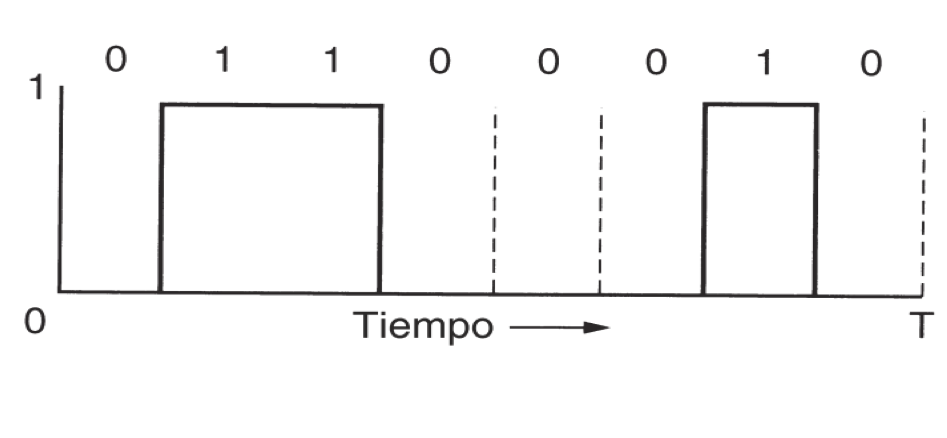
\includegraphics[width=6cm]{figs/06-bits.png}
  \end{center}
\end{frame}


%---------------------------------------------------------------------
\begin{frame}  
  \frametitle{Capa Física}

  Problema: la señal no es perfecta
  
  \begin{center}
    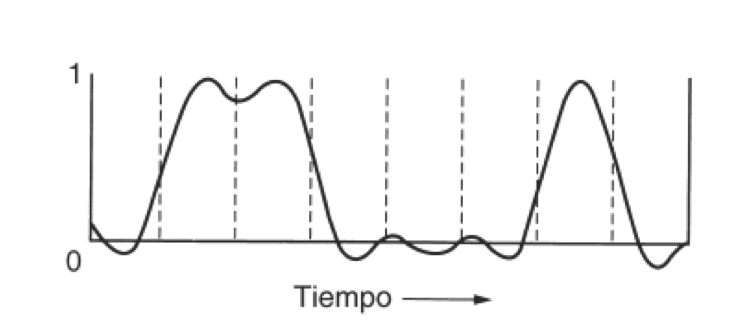
\includegraphics[width=6cm]{figs/06-bits-real.png}
  \end{center}
\end{frame}


%---------------------------------------------------------------------
\begin{frame}
  \frametitle{Series de Fourier}

  \begin{alertblock}{Jean-Baptiste Fourier, S.XIX}
    Cualquier función periódica $g(t)$, con periodo $T$ puede ser construida como una suma,
    posiblemente infinita, de senos y cosenos
    
    \[g(t) = \frac{1}{2}c + \sum^\infty_{n=1}a_n \sin(2\pi nft) + \sum^\infty_{n=1}b_n \cos(2\pi nft) \]
  \end{alertblock}
  
  donde:
  \begin{itemize}
    \item $f=1/T$ es la frecuencia fundamental
    \item $a_n$ y $b_n$ son las amplitudes de los $n$-ésimo armónicos
    \item $c$ es una constante
  \end{itemize}
  Conociendo $a_n$, $b_n$, $c$ y $T$, se puede reconstruir la función
\end{frame}

%---------------------------------------------------------------------
\begin{frame}
  \frametitle{¿Armónicos?}

  Múltiplos de una frecuencia fundamental
  
  \begin{center}
    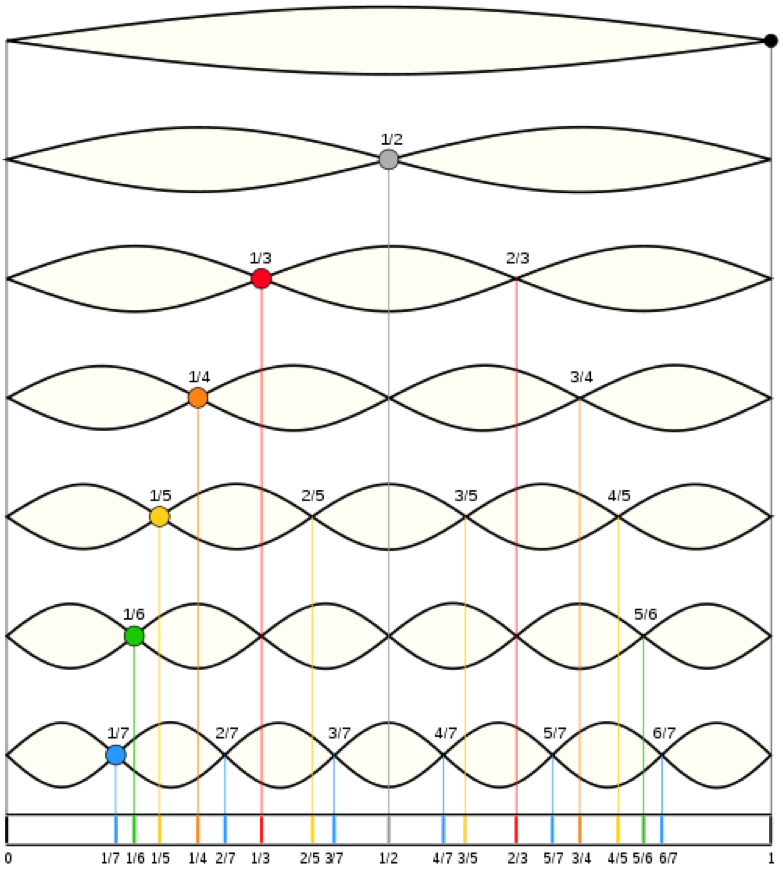
\includegraphics[width=6cm]{figs/06-armonicos.png}
  \end{center}
  

\end{frame}

%---------------------------------------------------------------------
\begin{frame}
  \frametitle{Sumando armónicos}

  Reconstruyendo señales
  
  \begin{center}
    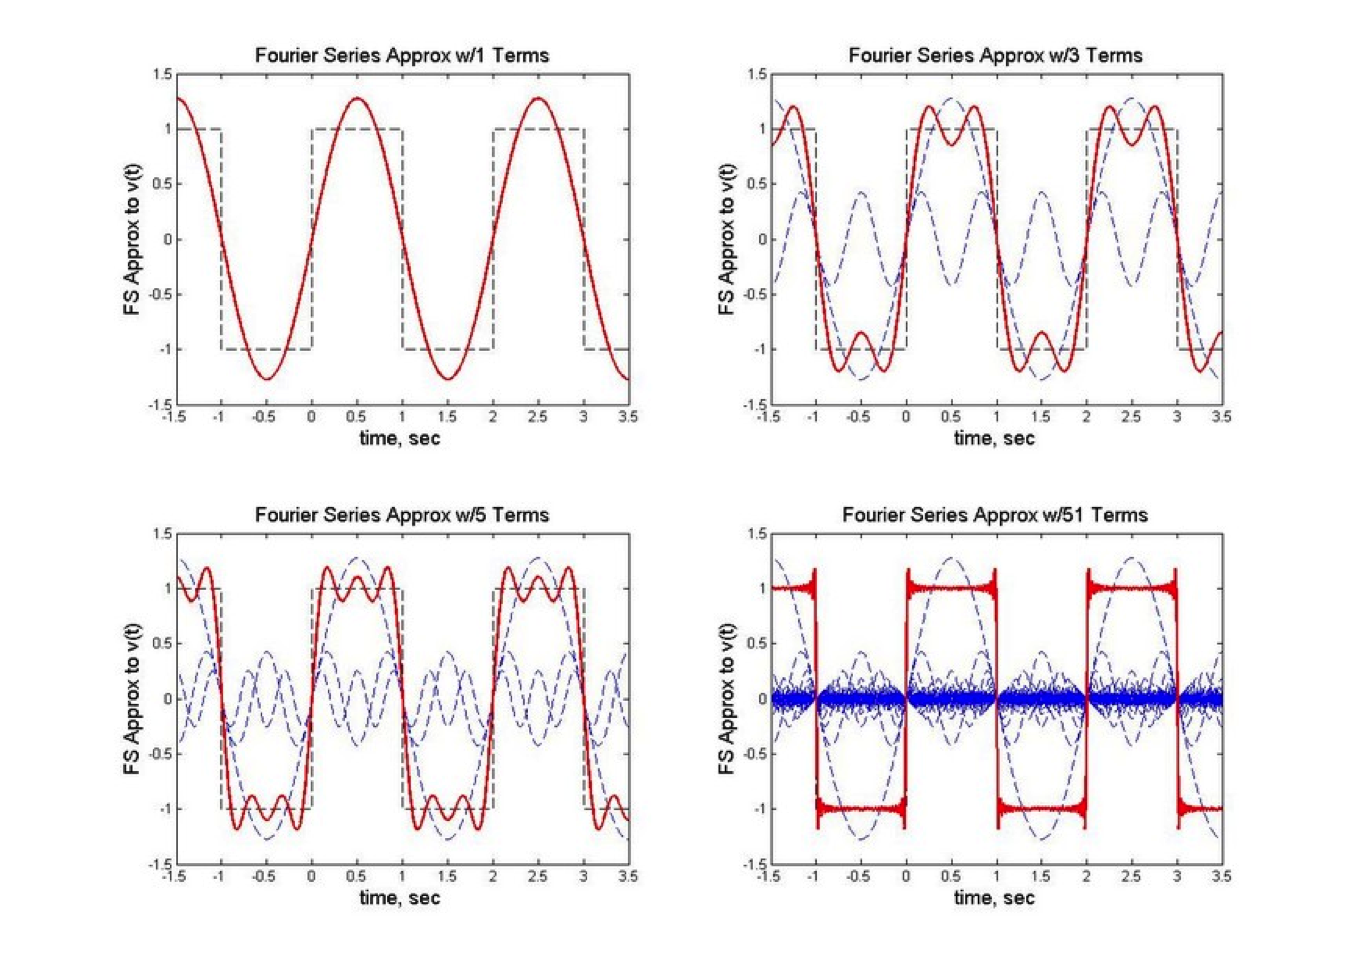
\includegraphics[width=10cm]{figs/06-fouriers.png}
  \end{center}
  

\end{frame}

%---------------------------------------------------------------------
\begin{frame}
  \frametitle{Reconstrucción de una señal}

  Ejemplo: Transmisión del caracter ASCII {\tt b}$=01100010$
  
  \begin{center}
    \includegraphics<1>[width=6cm]{figs/06-bits.png}
    \includegraphics<2>[width=10cm]{figs/06-fouriers-1.png}
    \includegraphics<3>[width=10cm]{figs/06-fouriers-2.png}
    \includegraphics<4>[width=10cm]{figs/06-fouriers-3.png}
    \includegraphics<5>[width=10cm]{figs/06-fouriers-4.png}
  \end{center}

\end{frame}
%---------------------------------------------------------------------
\subsection{Ancho de banda}

\begin{frame}
  \frametitle{Ancho de banda}

  Todos los medios sufren atenuación
  \begin{itemize}
    \item Hasta cierta frecuencia $f_c$ (en Hz) las amplitudes de los armónicos más altos se pierden
    \item La capacidad de frecuencias (harmónicos) que se pueden enviar por el canal
          sin ser (muy) atenuadas, determina el {\bf ancho de banda}
  \end{itemize}
  Si queremos enviar $8$-bit, a $b$ bits/sec (bps)
  \begin{itemize}
    \item Tiempo requerido: $8/b$ sec
    \item Frecuencia para primer armónico: $b/8$ Hz
    \item Línea telefónica transmite hasta $3000$ Hz
    \item Armónico más alto en línea telefónica: $3000/(b/8)=24000/b Hz$
  \end{itemize}

\end{frame}


%---------------------------------------------------------------------
\begin{frame}
  \frametitle{Ancho de banda}

  \begin{center}
    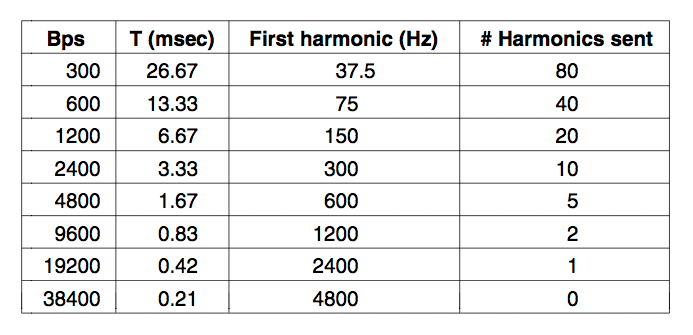
\includegraphics[width=10cm]{figs/06-bitrates.png}
  \end{center}

\end{frame}
%---------------------------------------------------------------------
\begin{frame}
  \frametitle{Ancho de banda máximo}

  Henry Nyquist (1924): Una señal con frecuencia $B$ puede ser completamente reconstruída
  tomando exactamente $2B$ muestra por segundo
  
  \begin{alertblock}{Teorema de Nyquist}
    \[\text{Máxima tasa de transferencia} = 2B \log_2 V \text{bps}\]
  \end{alertblock}
  
  donde:
  \begin{itemize}
    \item $B$: frecuencia máxima de la señal
    \item $V$: cantidad de niveles discretos
  \end{itemize}
  Ejemplo
  \begin{itemize}
    \item Canal perfecto de $3000$ Hz.
    \item Transmisión binaria, $V=2$
    \item Tasa máxima: $6000$ bps
  \end{itemize}

\end{frame}
%---------------------------------------------------------------------
\begin{frame}
  \frametitle{Ancho de banda máximo}

  Pero los canales tienen ruido.
  
  Claude Shannon (1948) presentó una fórmula para este caso
  
  \begin{alertblock}{Teorema de Shannon}
    \[\text{Máxima tasa de transferencia} = B \log_2 (1+\frac{S}{N}) \text{bps}\]
  \end{alertblock}
  donde:
  \begin{itemize}
    \item $S$: potencia de señal; $N$: potencia de ruido 
      \begin{itemize}
        \item $S/N$: SNR, Signal-to-Noise Ratio.
        \item Expresado en escala logarítimca: {\bf decibeles}
        \item $S/N=10=10\text{db}$;$100=20\text{db}$;$1000=30\text{db}$
      \end{itemize}
  \end{itemize}
  Ejemplo: línea ADSL sobre red telefónica: 1MHz
  \begin{itemize}
    \item Ancho de banda depende de SNR.
    \item SNR$=40$db, $1\sim 2$Km (bueno)
    \item Ancho de banda máximo: 13Mbps
  \end{itemize}

\end{frame}
%---------------------------------------------------------------------
\begin{frame}
  \frametitle{Espectro electromagnético}
  
  \begin{center}
    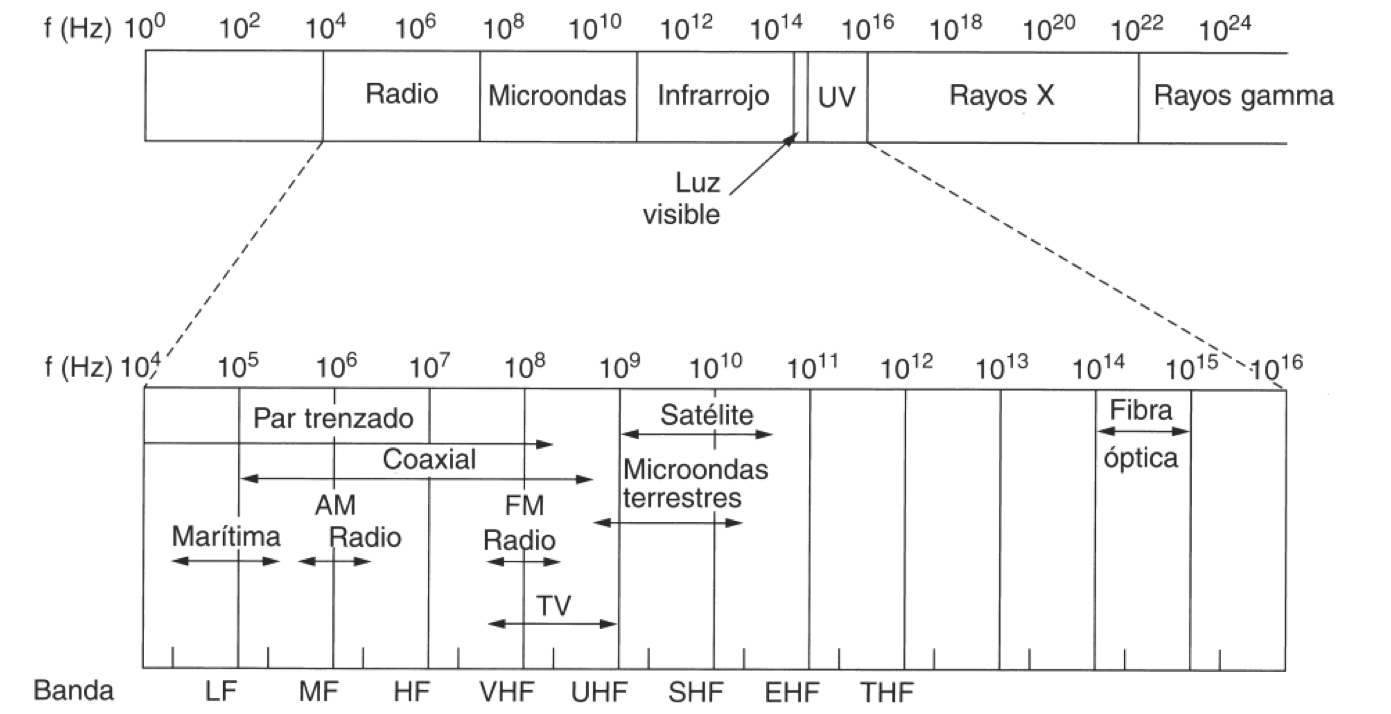
\includegraphics[width=10cm]{figs/06-espectro.png}
  \end{center}

\end{frame}

%---------------------------------------------------------------------
\subsection{Medios de transmisión}

\begin{frame}
  \frametitle{Cableado Estructurado}

  \begin{center}
    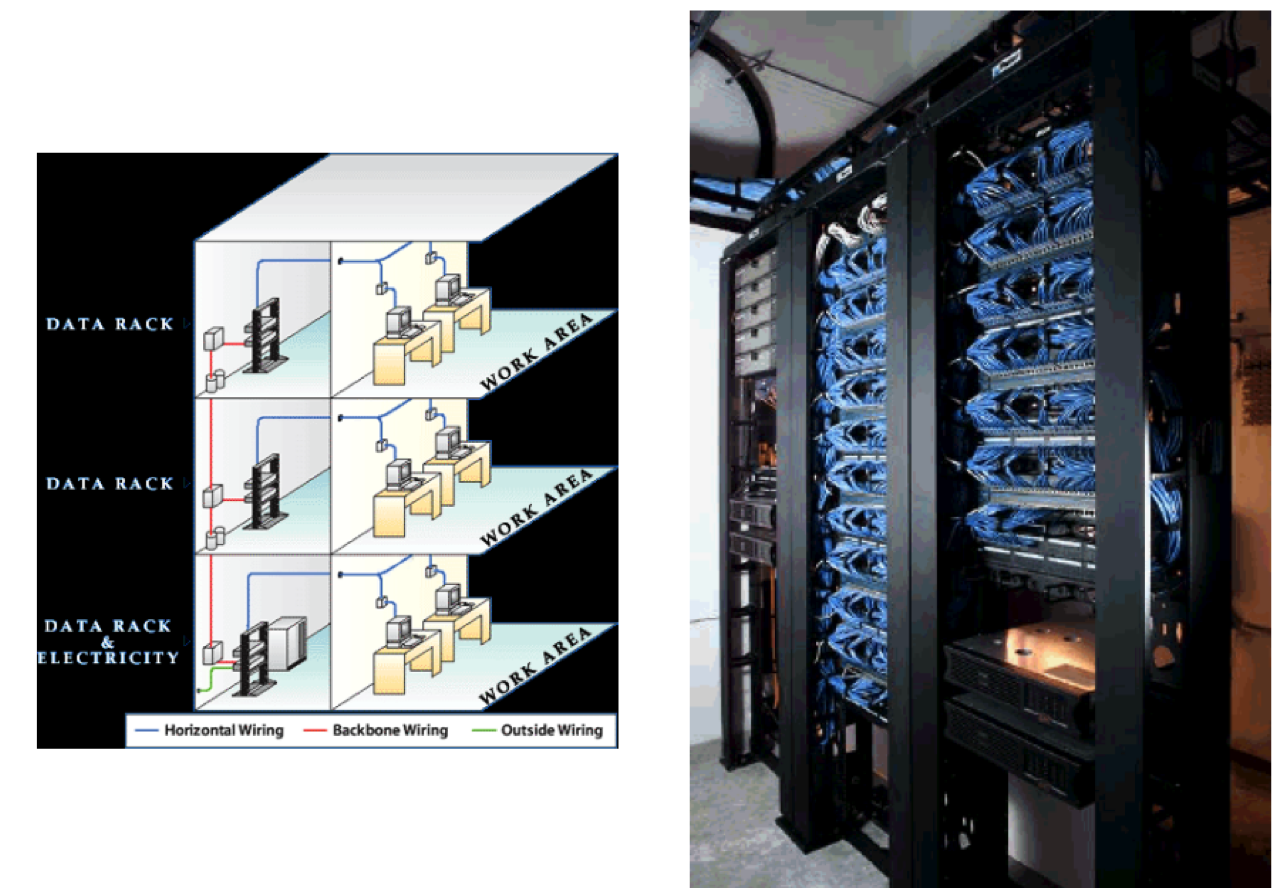
\includegraphics[width=10cm]{figs/06-cables.png}
  \end{center}

\end{frame}

%---------------------------------------------------------------------
\begin{frame}
  \frametitle{Cableado Estructurado}

  \begin{itemize}
    \item Cables trenzados se comportan como una antena
    \item Categorías según cuan trenzados estén: 3, 5, 5b, 6
    \item Recorren varios kilómetros ($\sim 5$km) sin atenuarse
  \end{itemize}
  \begin{center}
    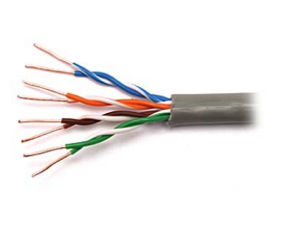
\includegraphics[width=5cm]{figs/06-trenzados.png}
  \end{center}
  Uso:
  \begin{itemize}
    \item Telefonía, ethernet
  \end{itemize}
\end{frame}
%---------------------------------------------------------------------
\begin{frame}
  \frametitle{Cableado Estructurado}
  
  Cable coaxial de cobre
  \begin{itemize}
    \item Alta resistencia al ruido externo
    \item Ancho de banda depende de la distancia
    \item Fácil de modificar para insertar nodos nuevos
    %\item Difícil detectar fallos
  \end{itemize}
  \begin{center}
    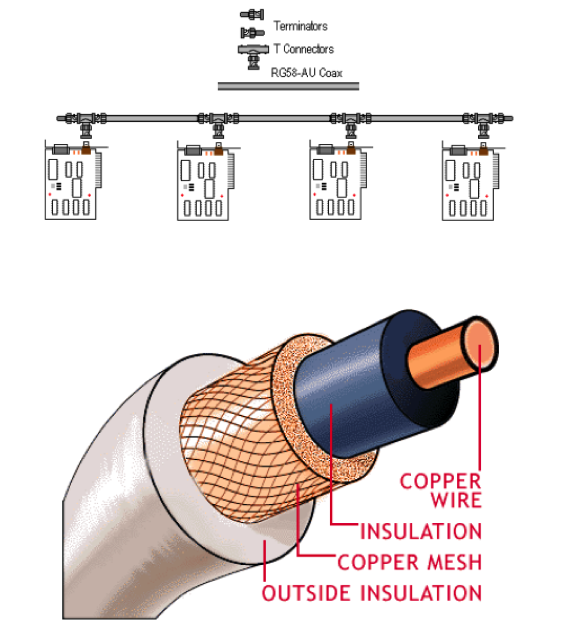
\includegraphics[width=4cm]{figs/06-coaxial.png}
  \end{center}

\end{frame}
%---------------------------------------------------------------------
\begin{frame}
  \frametitle{Cableado Estructurado}

  Fibra óptica
  \begin{itemize}
    \item Transmisión y detección de luz
    \item Cables hechos de vidrio
    \item Alta velocidad de transferencia
  \end{itemize}
  \begin{center}
    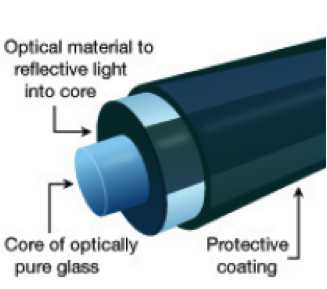
\includegraphics[width=2cm]{figs/06-fibra1.png}
  \end{center}
  \begin{itemize}
    \item Monomodo: un haz de luz
    \item Multimodo: múltiples haces a distintos ángulos
  \end{itemize}
  \begin{center}
    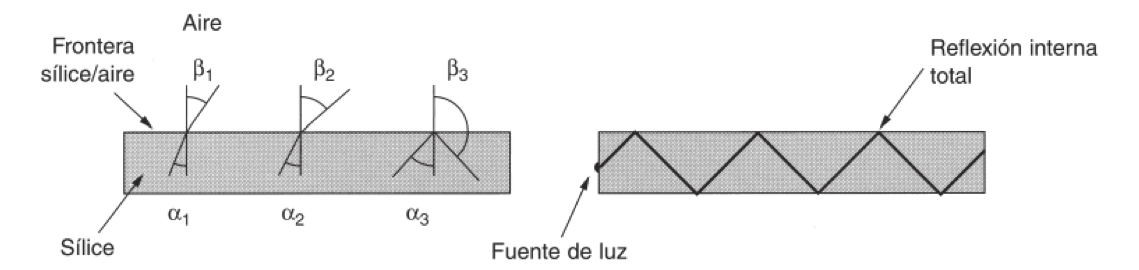
\includegraphics[width=7cm]{figs/06-fibra2.png}
  \end{center}
\end{frame}
%---------------------------------------------------------------------
\begin{frame}
  \frametitle{Medios Inalámbricos}

  Satélites
  
  \begin{itemize}
    \item Comunicación de larga distancia
    \item Configuraciones
      \begin{itemize}
        \item Geoestacionaria
        \item Órbita media (MEO): GPS ($\sim 32$)
        \item Órbita baja (LEO):  
      \end{itemize}
    \item Velocidad de transmisión: $\sim 300000$km/s
    \item Comunicación puede apoyarse en medios terrestres
  \end{itemize}

\end{frame}
%---------------------------------------------------------------------
\begin{frame}
  \frametitle{Medios Inalámbricos}

  \begin{center}
    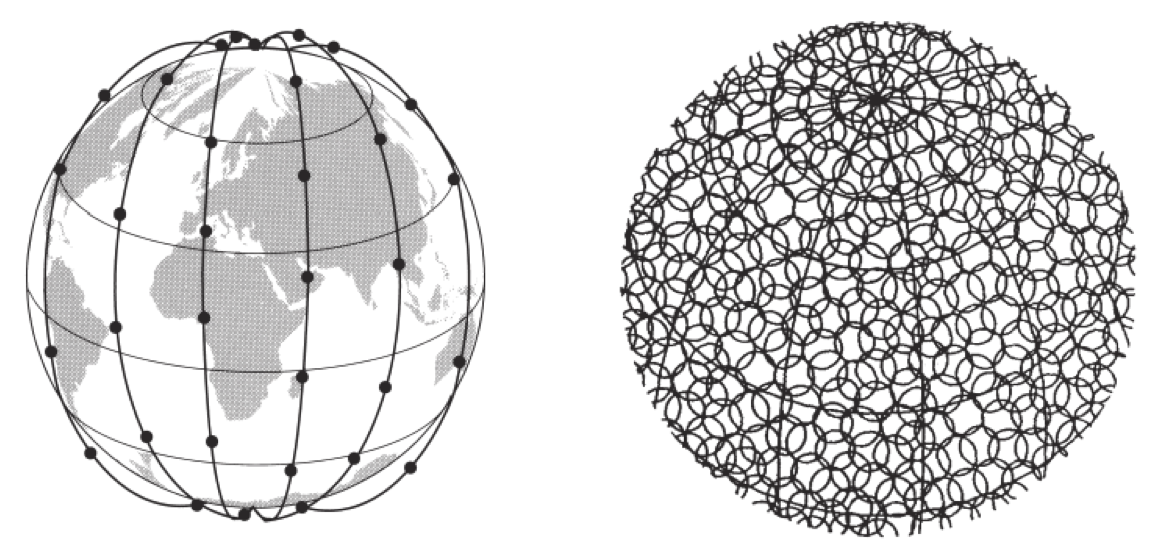
\includegraphics[width=7cm]{figs/06-satelite1.png}
  \end{center}

  \begin{center}
    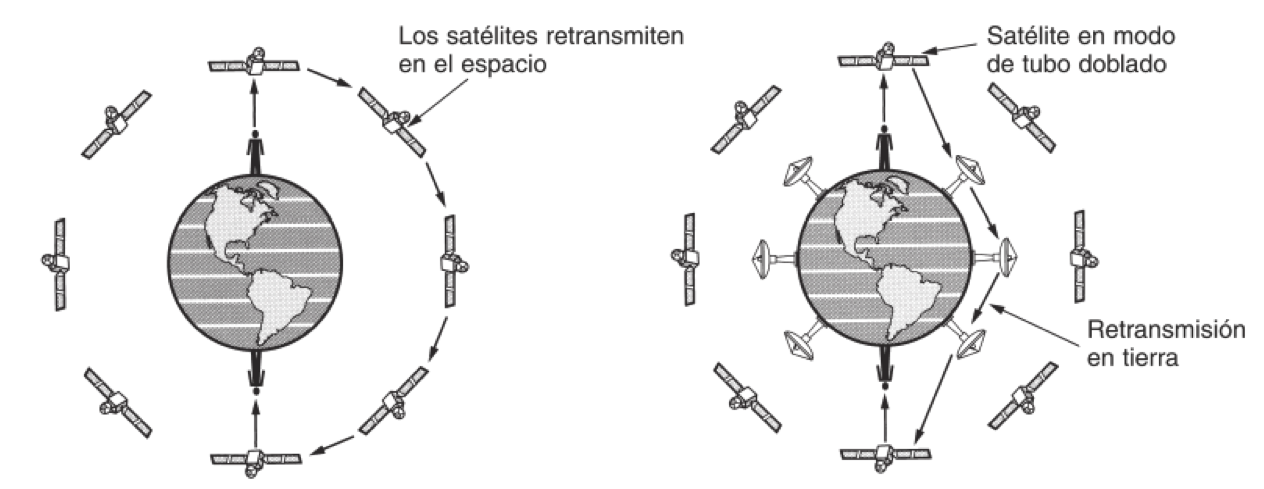
\includegraphics[width=7cm]{figs/06-satelite2.png}
  \end{center}
  

\end{frame}
%---------------------------------------------------------------------
\begin{frame}
  \frametitle{Medios Inalámbricos}

  Medios inalámbricos ``terrestres''
  \begin{itemize}
    \item Señal se debilita en el aire al propagarse
    \item Interferencia con otras señales: asignación de frecuencias
    \item Propagación multicamino: señales llegan por distintos caminos
  \end{itemize}

\end{frame}

%---------------------------------------------------------------------
\begin{frame}
  \frametitle{Medios Inalámbricos}

  Estándares de comunicación inalámbrica
  
  \begin{center}
    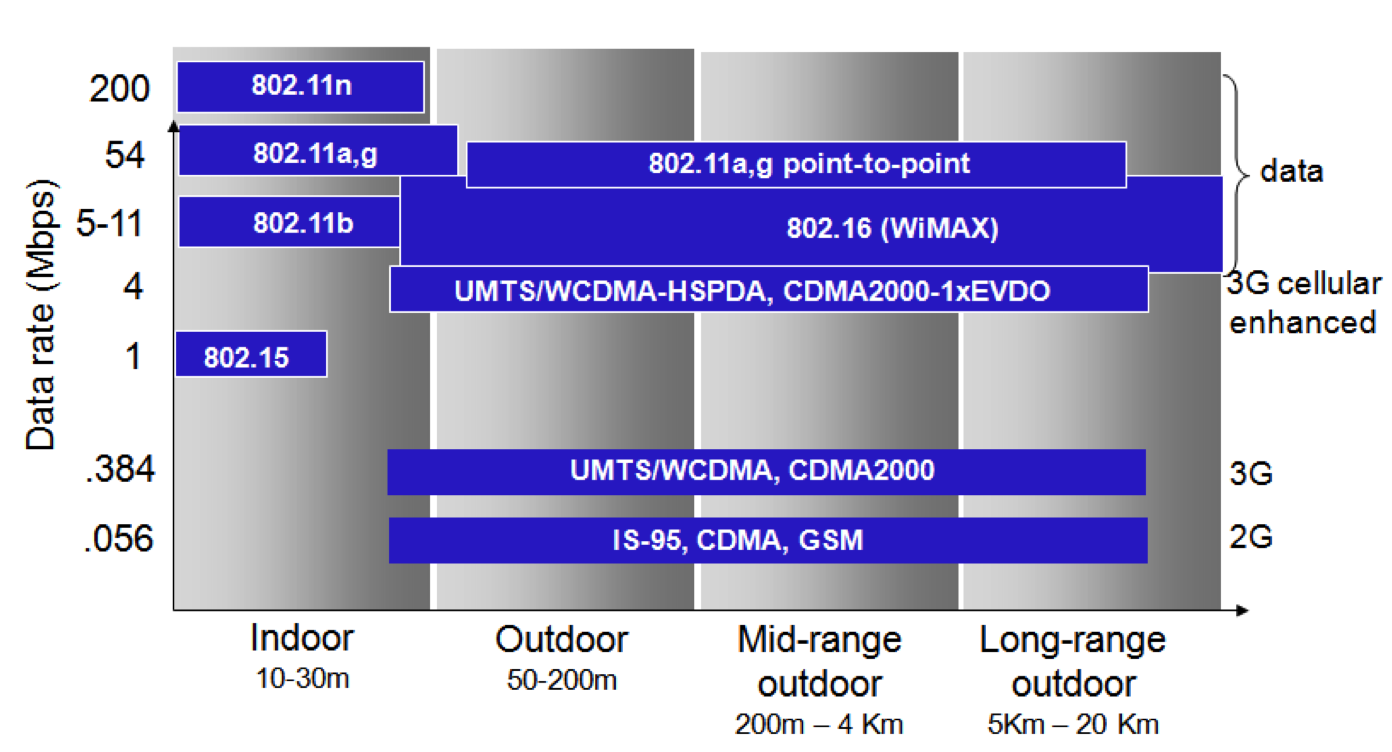
\includegraphics[width=10cm]{figs/06-wireless.png}
  \end{center}
  

\end{frame}

%---------------------------------------------------------------------
\begin{frame}
  \frametitle{Medios Inalámbricos}

  IEEE 802.11, Wireless LAN
  
  \begin{itemize}
    \item 802.11b, $2.4\sim 2.5$GHz, 11 Mbps
    \item 802.11a, $5 \sim 6$GHz, 54 Mbps, sensible a interferencias físicas
    \item 802.11g, $2.4\sim 2.5$GHz, 54 Mbps
    \item 802.11n, $2.4\sim 2.5$GHz, 200 Mbps, múltiples antenas
  \end{itemize}

\end{frame}
%---------------------------------------------------------------------
\begin{frame}
  \frametitle{Medios Inalámbricos}
  \framesubtitle{IEEE 802.11, Wireless LAN}

  \begin{center}
    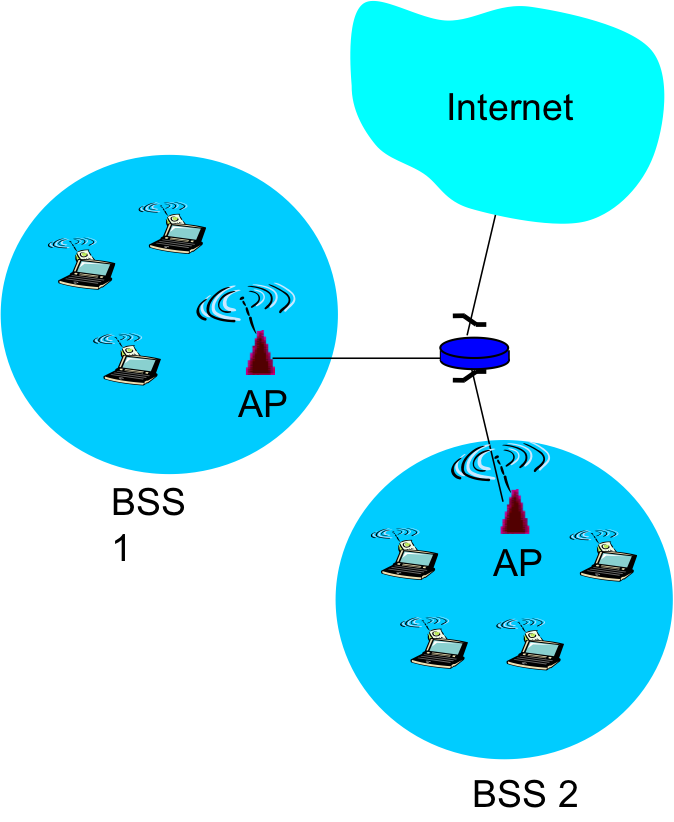
\includegraphics[width=4cm]{figs/06-wlan.png}
  \end{center}

  \begin{itemize}
    \item Estación base: {\em Access Point} (AP)
    \item BSS: Basic Service Set
    \item Modos de operación: {\em infrastructure} y {\em ad-hoc}
  \end{itemize}
  
\end{frame}
%---------------------------------------------------------------------
\begin{frame}
  \frametitle{Medios Inalámbricos}
  \framesubtitle{IEEE 802.11, Wireless LAN}

  Canales. Espectro 2.4GHz $\sim$ 2.485GHz dividido en 11 canales
  
  \begin{itemize}
    \item Administrador de AP elige el canal
    \item {\em Host} escucha canales y detecta {\em beacons} enviados por AP
    \item {\em Beacons} contienen SSID (nombre de AP) y MAC Address de AP
  \end{itemize}  

  \begin{center}
    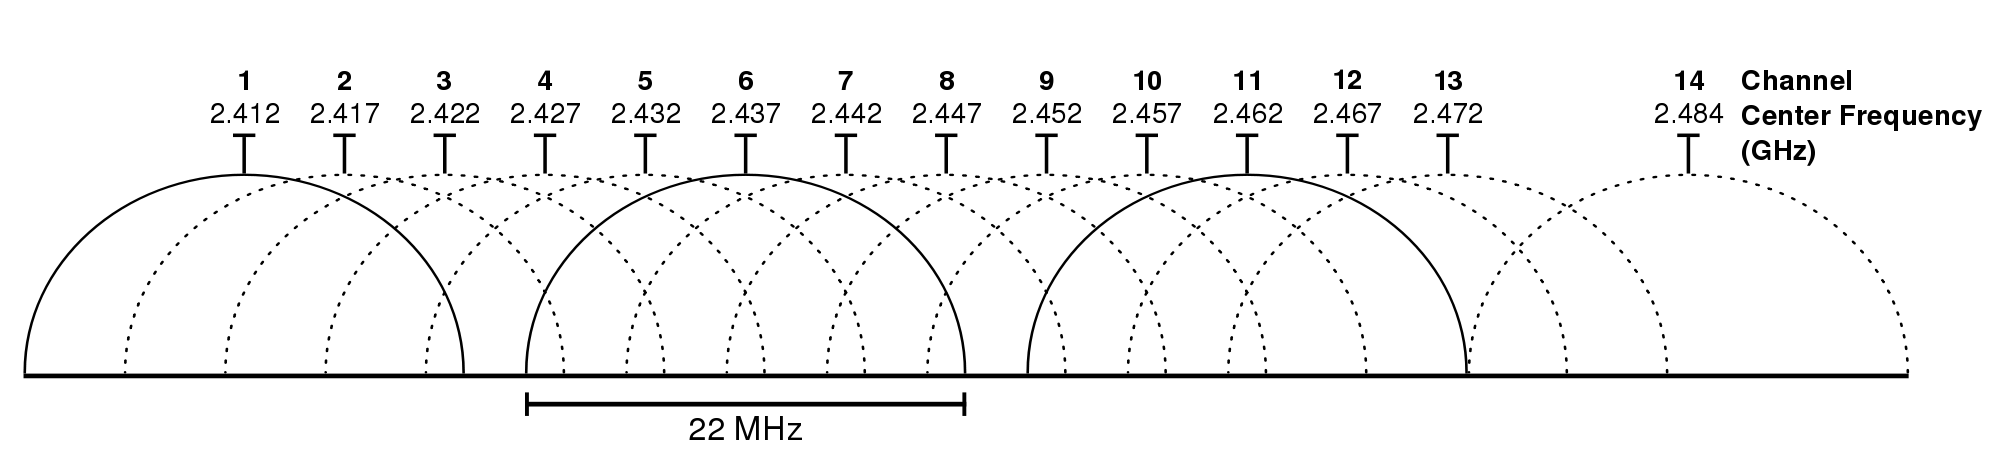
\includegraphics[width=11cm]{figs/06-channels.png}
  \end{center}

\end{frame}
%---------------------------------------------------------------------
\begin{frame}
  \frametitle{Medios Inalámbricos}
  \framesubtitle{IEEE 802.16, WiMax}

  \begin{itemize}
    \item Comunicación base-hosts: antena omnidireccional
    \item Comunicación base-base: antena punto a punto
    \item Rango $\sim$ 10Km, $\sim$ 14Mbps
  \end{itemize}

  \begin{center}
    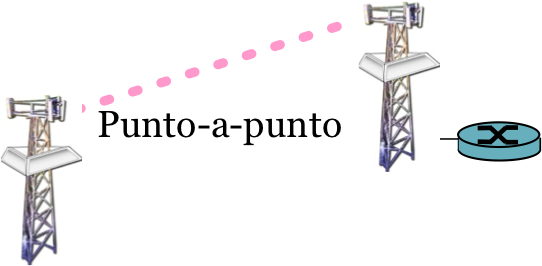
\includegraphics[width=4cm]{figs/06-wimax1.png}
    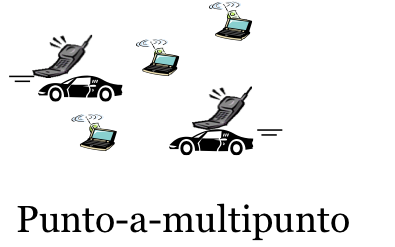
\includegraphics[width=4cm]{figs/06-wimax2.png}
    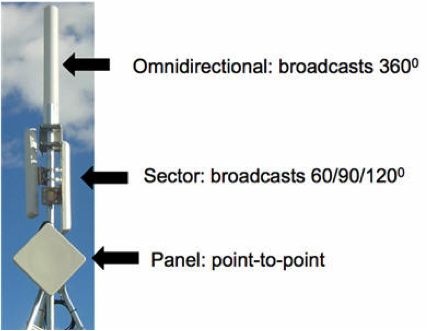
\includegraphics[width=4cm]{figs/06-wimax3.png}
  \end{center}


\end{frame}

%---------------------------------------------------------------------
\begin{frame}
  \frametitle{Medios Inalámbricos}
  \framesubtitle{Red Móvil 2G}

  \begin{itemize}
    \item Canales de voz
    \item IS-136: TDMA + FDMA (Time Division/Freq Division)
    \item GSM: Global System for Telecommunications
    \item IS-95: CDMA (Code Division Multiple Access)
  \end{itemize}
  
\end{frame}
%---------------------------------------------------------------------
\begin{frame}
  \frametitle{Medios Inalámbricos}
  \framesubtitle{Red Móvil 2.5G}

  \begin{itemize}
    \item GPRS: General Packet Radio Service
      \begin{itemize}
        \item GSM++
        \item Envío de datos
      \end{itemize}
    \item EDGE: Enhanced Data rates for Global Evolution
      \begin{itemize}
        \item Data rates hasta 384Kbps
      \end{itemize}
  \end{itemize}
  

\end{frame}

%---------------------------------------------------------------------
\begin{frame}
  \frametitle{Medios Inalámbricos}
  \framesubtitle{Red Móvil 3G}

  Voz + Datos
  
  \begin{itemize}
    \item UMTS: Universal Mobile Telecommunications Service
      \begin{itemize}
        \item WCDMA
        \item HSPA+, High Speed Packet Access (evolved): 168Mbps downlink, 22Mbps uplink
      \end{itemize}
    \item CDMA-2000: CDMA en slots TDMA
  \end{itemize}

\end{frame}

%---------------------------------------------------------------------
\section{Frames, control de flujo, corrección de errores}

\begin{frame}
  \frametitle{Capa de Enlace}
  
  Objetivo: transmitir datos de la capa de red a través un enlace particular
  
  \begin{itemize}
    \item Unidad de transmisión: {\bf frame}
  \end{itemize}
  
  Desafíos:
  \begin{itemize}
    \item Múltiples nodos intentando acceder a un medio compartido
    \item Cómo asegurar que un {\bf frame} llegue íntegramente: {\bf detección de errores}
    \item Qué hacer si un {\em host} llega a un punto de saturación y no puede recibir/emitir más frames:
          {\bf control de flujo}
  \end{itemize}

\end{frame}

%---------------------------------------------------------------------
\begin{frame}
  \frametitle{Capa de Enlace}
  
  \begin{itemize}
    \item Datos de capa de red se encapsula en un {\em frame} delimitado
          por {\em header} y {\em trailer}
    \item Identificación de {\em hosts} de origen y destino: {\bf MAC Address}
  \end{itemize}
\end{frame}

%---------------------------------------------------------------------
\begin{frame}
  \frametitle{Capa de Enlace}

  Detección de errores
  \begin{itemize}
    \item No utilizado en medios de baja tasa de error (fibra, cables)
    \item Importante en medios con atenuación (inalámbricos)
      \begin{itemize}
        \item Receptor detecta errores por atenuación 
        \item Solicita retransmisión, o desecha {\em frame}
        \item Si se agrega código de corrección, receptor puede corregir
      \end{itemize}
  \end{itemize}

\end{frame}
%---------------------------------------------------------------------
\begin{frame}
  \frametitle{Capa de Enlace}

  ¿Dónde se implementa?
  
  \begin{itemize}
    \item {\bf Network Interface Card} (NIC)
  \end{itemize}

  \begin{center}
    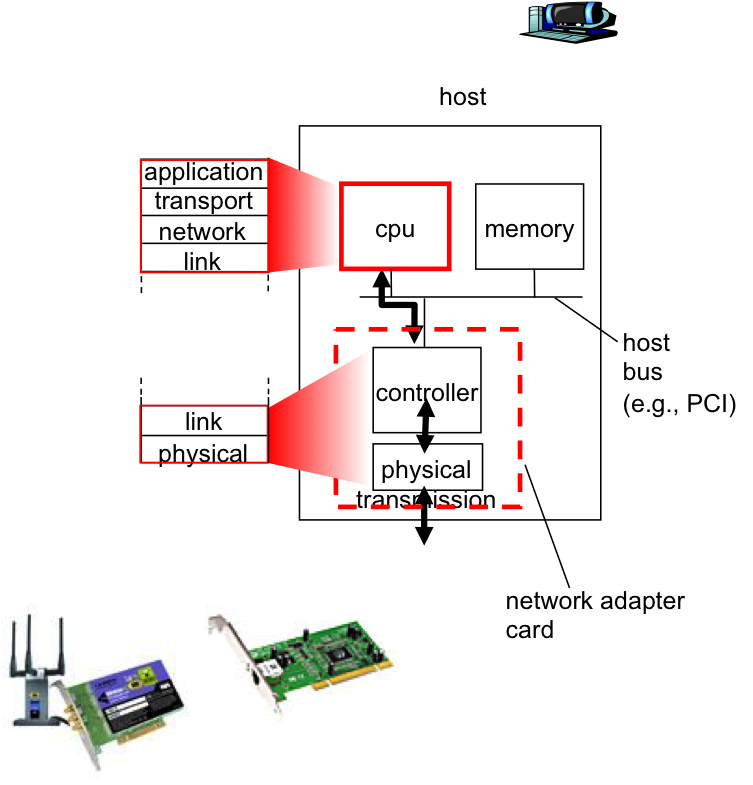
\includegraphics[width=6cm]{figs/06-nic.png}
  \end{center}

\end{frame}

%---------------------------------------------------------------------
\begin{frame}
  \frametitle{Frame {\em Ethernet}}

  \begin{center}
    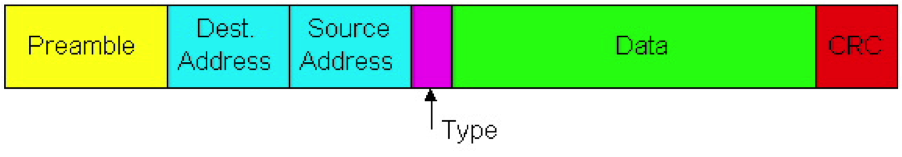
\includegraphics[width=10cm]{figs/06-frameethernet.png}
  \end{center}

  \begin{itemize}
    \item {\bf Preámbulo}
      \begin{itemize}
        \item 7 bytes 10101010, + 1 byte 10101011
        \item Usado para sincronizar relojes de emisor y receptor
      \end{itemize}
    \item {\bf Direcciones}: 6 bytes
    \item {\bf Tipo}: indica protocolo de capa de red
    \item {\bf CRC}: Cyclic Redundancy Check, comprobación de errores
  \end{itemize}
  
\end{frame}

%---------------------------------------------------------------------
\begin{frame}
  \frametitle{Frame {\em WLAN}}

  \begin{center}
    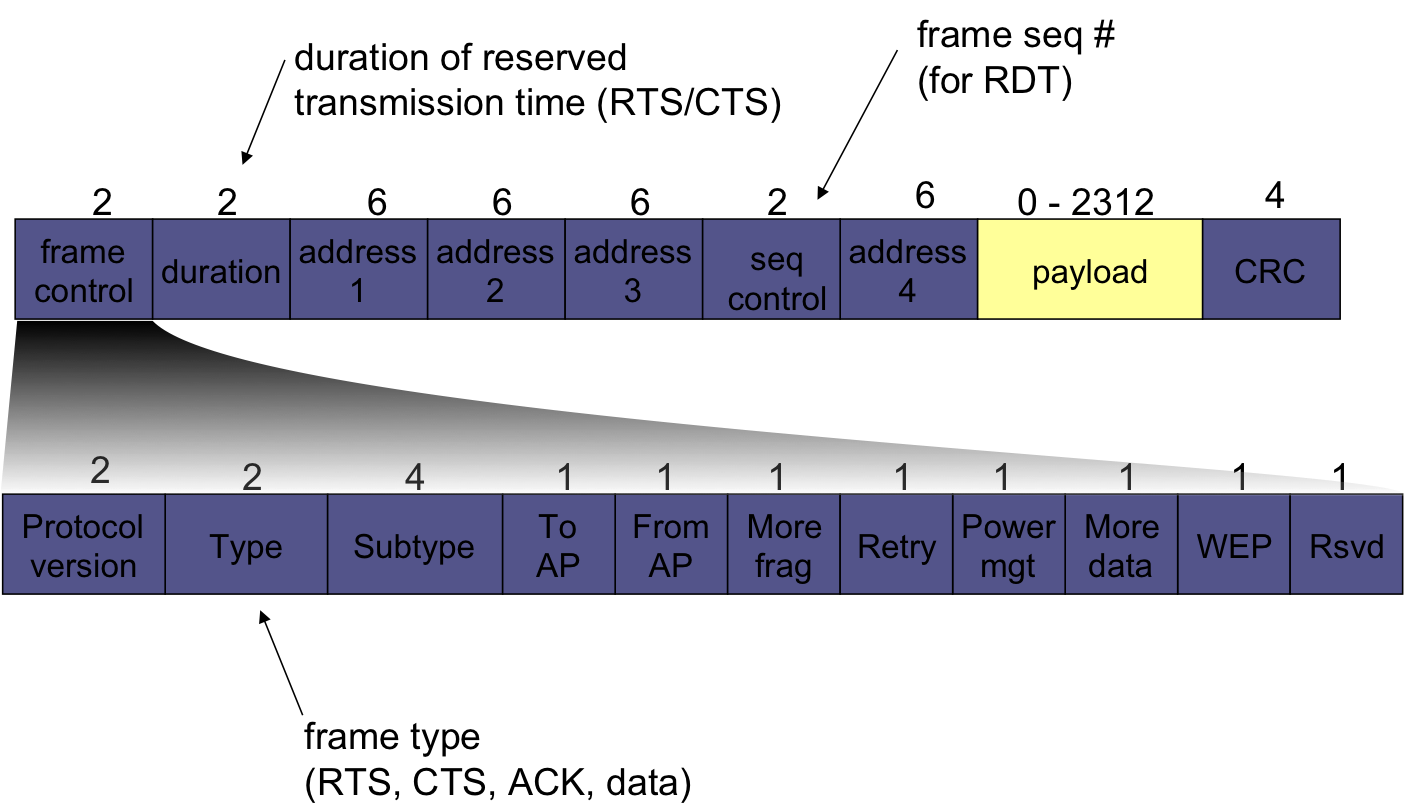
\includegraphics[width=11cm]{figs/06-framewlan.png}
  \end{center}

\end{frame}

%---------------------------------------------------------------------
\begin{frame}
  \frametitle{Detección de errores}
  \framesubtitle{Shit happens}
  
  ¿Cómo saber si un {\em frame} llegó con errores?
  
  \begin{itemize}
    \item Se agregan bits de ``comprobación'' que ayuden a detectar algunos errores.
  \end{itemize}

  \begin{center}
    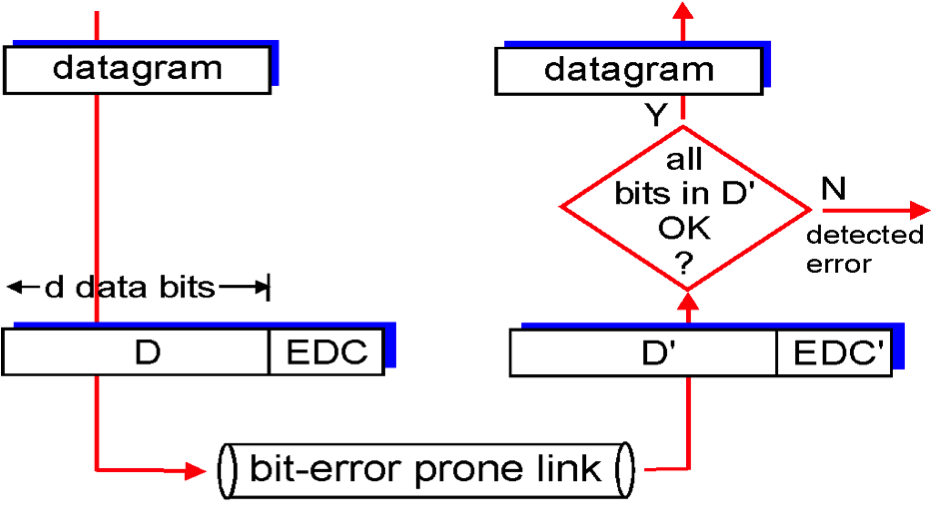
\includegraphics[width=9cm]{figs/06-errordetection.png}
  \end{center}


\end{frame}

%---------------------------------------------------------------------
\begin{frame}
  \frametitle{Detección de errores}
  \framesubtitle{Bits de paridad}

  \begin{itemize}
    \item Paridad simple. Para detectores errores de un bit
      \begin{center}
        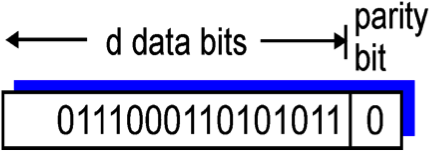
\includegraphics[width=3cm]{figs/06-paritysimple.png}
      \end{center}
    \item Paridad doble. Para detectar {\bf y corregir} errores de un bit
      \begin{center}
        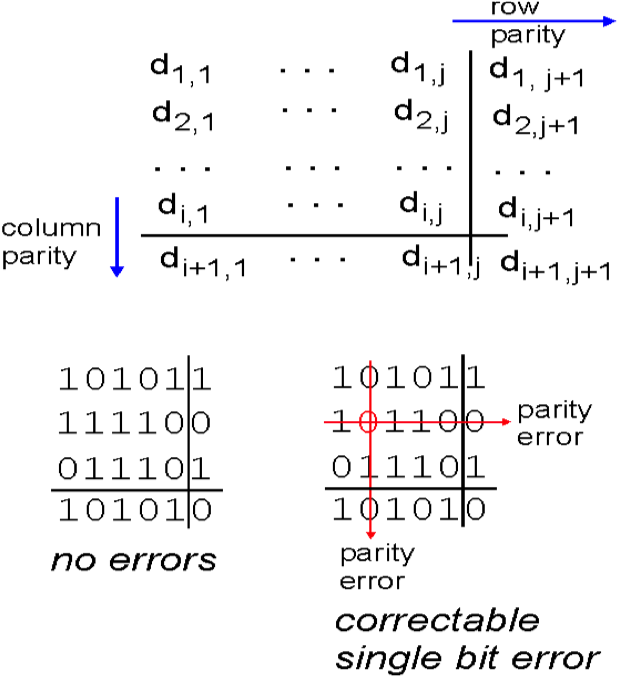
\includegraphics[width=4cm]{figs/06-paritydouble.png}
      \end{center}
  \end{itemize}

\end{frame}

%---------------------------------------------------------------------
\begin{frame}
  \frametitle{CRC: {\em Cyclic Redundancy Check}}
  \framesubtitle{Comprobación de Redundancia Cíclica}

  \begin{itemize}
    \item $D$: secuencia de $d$ bit de datos
    \item $R$: secuencia de $r$ bit de comprobación (CRC)
    \item Se usa un patrón conocido $G$, de $r+1$ bit
    \begin{itemize}
      \item La secuencia $\langle D,R \rangle$ debe ser divisible por $G$
      \item Receptor puede chequear el resto de dividir $\langle D,R \rangle$ por $G$
      \item Esquema detecta errores de hasta $r$ bit
    \end{itemize}
    \item Teoría: 
      \begin{itemize}
        \item $(D\times 2^r) \oplus R = nG$
        \item $(D\times 2^r) = nG \oplus R$
        \item $R$ es el resto de la división binaria $\frac{D \times 2^r}{G}$
      \end{itemize}
  \end{itemize}
  
\end{frame}

%---------------------------------------------------------------------
\begin{frame}
  \frametitle{CRC: {\em Cyclic Redundancy Check}}
  \framesubtitle{Comprobación de Redundancia Cíclica}

  Ejemplo: $D=101110$, $G=1001$, determinar $R$
  
  \begin{tabular}{ccccccccc}
    1 & 0 & 1 & 1 & 1 & 0 & 0 & 0 & 0 \\
    1 & 0 & 0 & 1 &   &   &   &   &   \\ \hline
    0 & 0 & 1 & 0 & 1 & 0 & 0 & 0 & 0 \\
      &   & 1 & 0 & 0 & 1 &   &   &   \\ \hline
      &   & 0 & 0 & 1 & 1 & 0 & 0 & 0 \\
      &   &   &   & 1 & 0 & 0 & 1 &   \\ \hline
      &   &   &   & 0 & 1 & 0 & 1 & 0 \\
      &   &   &   &   & 1 & 0 & 0 & 1 \\ \hline
      &   &   &   &   & 0 & 0 & 1 & 1 \\ \hline
  \end{tabular}
  $R = 011$
  \begin{itemize}
    \item Se envía: $101110011$
  \end{itemize}
  Paridad simple es un caso particular, con $G=1$
\end{frame}

%---------------------------------------------------------------------
\section{Acceso al medio: ethernet y wireless LAN}

\begin{frame}
  \frametitle{Acceso al medio: MAC}
  \framesubtitle{{\em Medium Access Control}}
  
  Problema: múltiples usuarios requieren acceso a un medio
  \begin{itemize}
    \item Importante para medios compartidos ({\em broadcast})
  Tres tipos de soluciones
  \begin{itemize}
    \item Partición de canal: tiempo, frecuencia o código
    \item Acceso aleatorio
    \item Turnos
  \end{itemize}
    
  \end{itemize}

\end{frame}

%---------------------------------------------------------------------
\begin{frame}
  \frametitle{Partición de canal: TDMA}
  \framesubtitle{{\em Time Division Multiple Access}}

  \begin{itemize}
    \item Acceso por turnos fijos
    \item Cada nodo tiene un {\em slot} que es múltiplo de un periodo de tiempo
      \begin{itemize}
        \item Con $N$ nodos y {\em slot} de tiempo $T$, se hacen rondas de $NT$
        \item Nodo $i$ durante $[(rN+i)\times T, (rN+i+1)\times T)$
        \item Con 6 nodos de 5 sec, nodo 0 transmite durante $[0,5), [30,35), [60,65), \ldots$
      \end{itemize}
    \item {\em Slot}s no utilizados se pierden
  \end{itemize}
  
  \begin{center}
    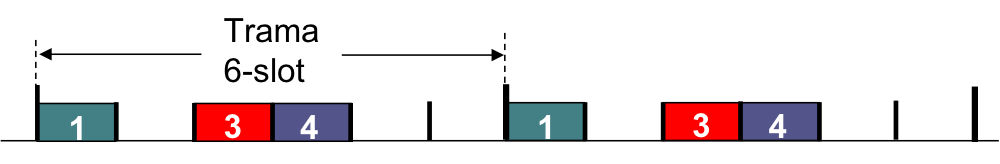
\includegraphics[width=7cm]{figs/06-tdma.png}
  \end{center}


\end{frame}
%---------------------------------------------------------------------
\begin{frame}
  \frametitle{Partición de frecuencia: FDMA}
  \framesubtitle{{\em Frequency Division Multiple Access}}

  \begin{itemize}
    \item División por bandas de frecuencia. (Ej: canales de radio, televisión)
    \item Cada estación tiene una banda fija asignada
    \item Bandas no utilizadas quedan inactivas
  \end{itemize}

  \begin{center}
    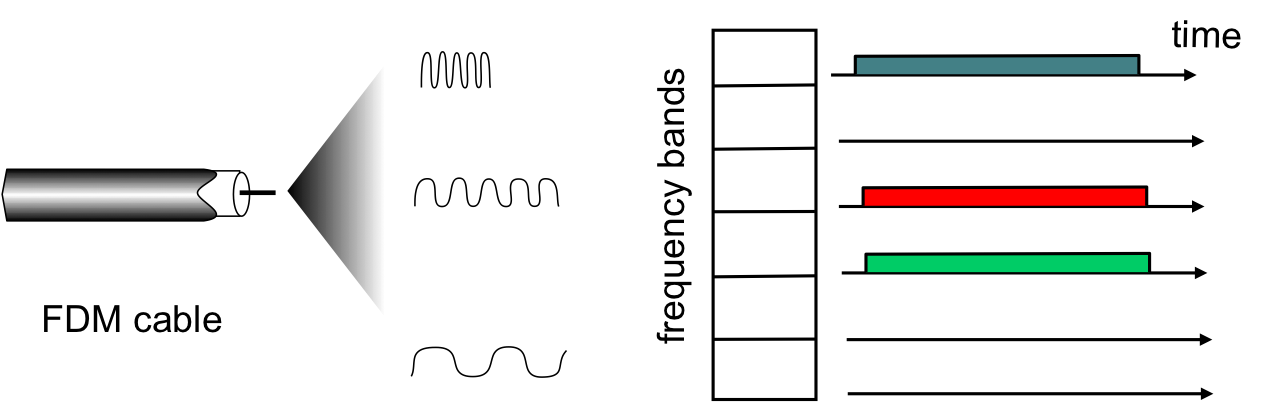
\includegraphics[width=8cm]{figs/06-fdma.png}
  \end{center}

\end{frame}
%---------------------------------------------------------------------
\begin{frame}
  \frametitle{División por código: CDMA}
  \framesubtitle{{\em Code Division Multiple Access}}

  \begin{itemize}
    \item Permite que varios usuarios transmitan en la misma frecuencia
    \item Cada usuario posee un código de transmisión
      \begin{itemize}
        \item Requisito: códigos deben ser ortogonales
        \item Señal a transmitir: {\em data cliente} $ \cdot $ {\em código cliente}
        \item Señal recibida: {\em data recibida} $ \cdot $ {\em código cliente}
      \end{itemize}
  \end{itemize}

\end{frame}

%---------------------------------------------------------------------
\begin{frame}
  \frametitle{División por código: CDMA}
  \framesubtitle{{\em Code Division Multiple Access}}

  \begin{center}
    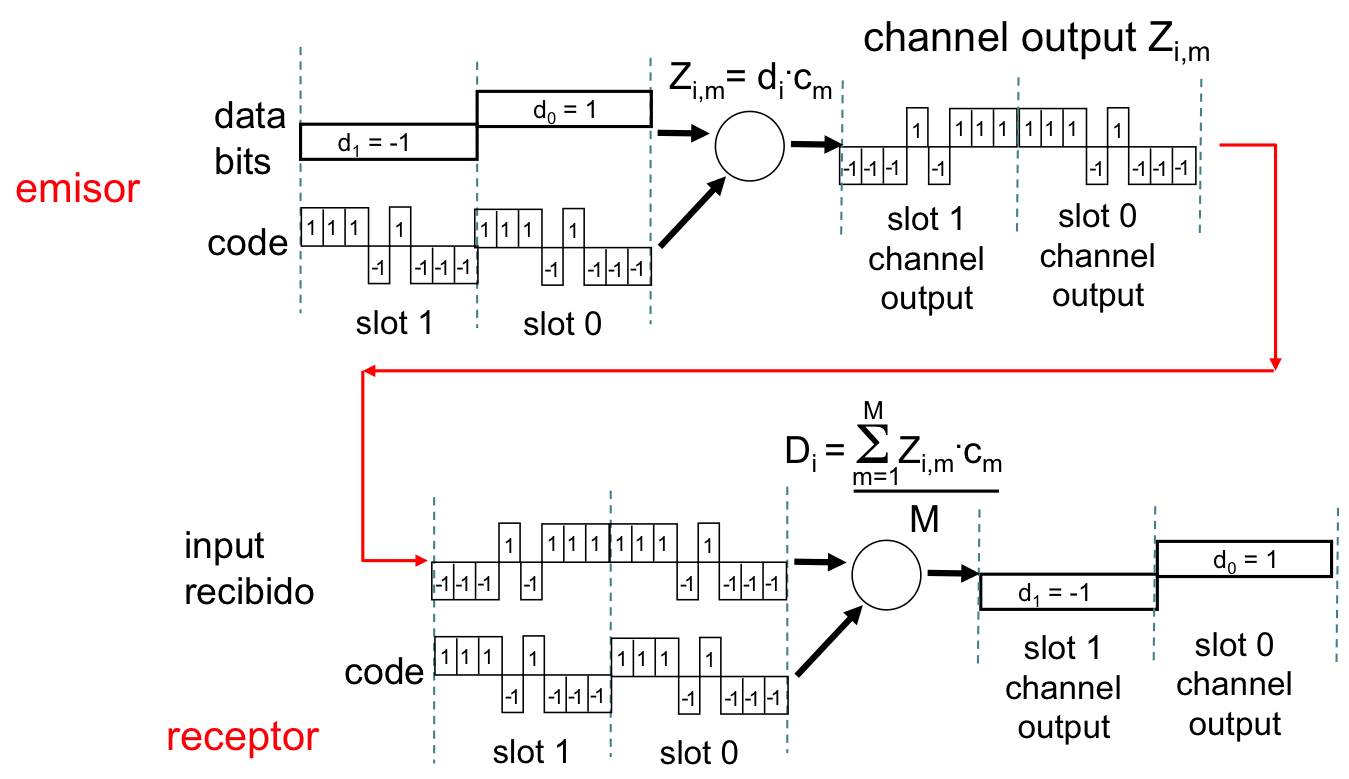
\includegraphics[width=10cm]{figs/06-cdma1.png}
  \end{center}

\end{frame}

%---------------------------------------------------------------------
\begin{frame}
  \frametitle{División por código: CDMA}
  \framesubtitle{{\em Code Division Multiple Access}}

  \begin{center}
    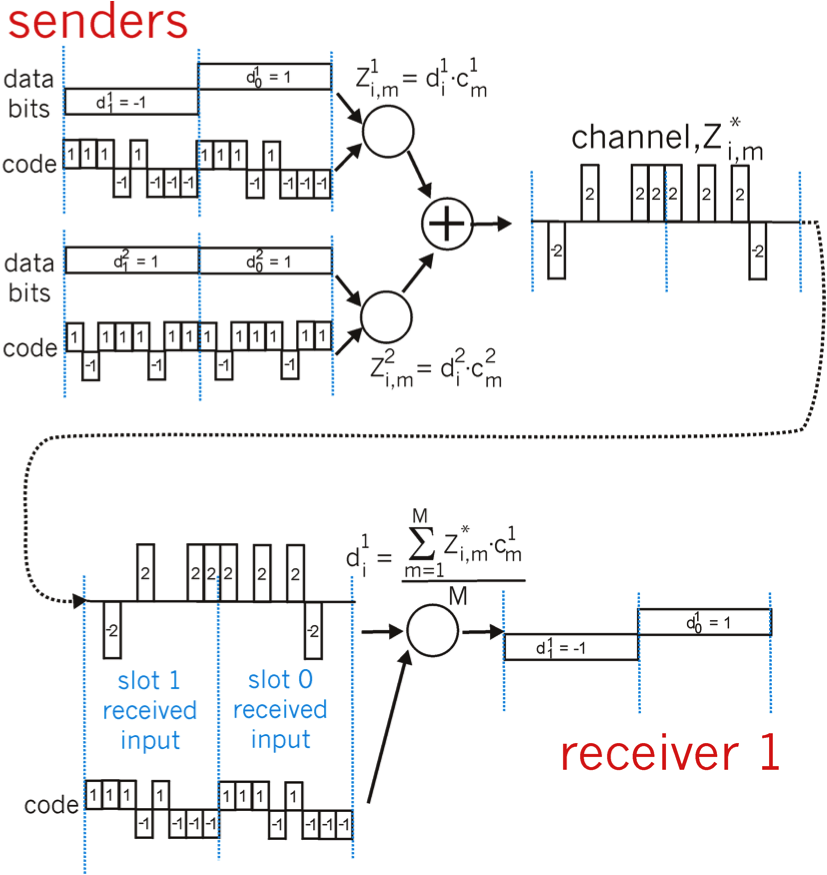
\includegraphics[width=7cm]{figs/06-cdma2.png}
  \end{center}

\end{frame}
%---------------------------------------------------------------------
\begin{frame}
  \frametitle{Acceso Aleatorio}
  \framesubtitle{Todos hablan cuando quieren}

  Protocolos optimistas
  \begin{itemize}
    \item Cada nodos transmite cuando lo desea ocupando todo el ancho de banda disponible
    \item Si dos o más transmite al mismo tiempo, se produce {\bf colisión}
    \item Protocolo debe determinar:
      \begin{itemize}
        \item Cómo detectar colisiones
        \item Qué hacer ante una colisión (cómo recuperarse)
      \end{itemize}
    \item Protocolos:
      \begin{itemize}
        \item ALOHA particionado
        \item ALOHA
        \item CSMA, CSMA/CD, CSMA/CA
      \end{itemize}
  \end{itemize}

\end{frame}
%---------------------------------------------------------------------
\begin{frame}
  \frametitle{ALOHA Particionado}
%  \framesubtitle{Todos hablan cuando quieren}

  \begin{itemize}
    \item Todos los frames deben tener el mismo tamaño
    \item El tiempo se divide en particiones del tamaño requerido para transmitir un frame
    \item Nodos pueden empezar a transmitir sólo al comienzo de estas particiones
    \item Si dos o más empiezan a transmitir en la misma partición, se detecta {\bf colisión}
  \end{itemize}
  Ante una colisión:
  \begin{itemize}
    \item Cada nodo vuelve a transmitir en la siguiente partición, con probabilidad $p$, hasta que no haya colisiones
  \end{itemize}
  \begin{center}
    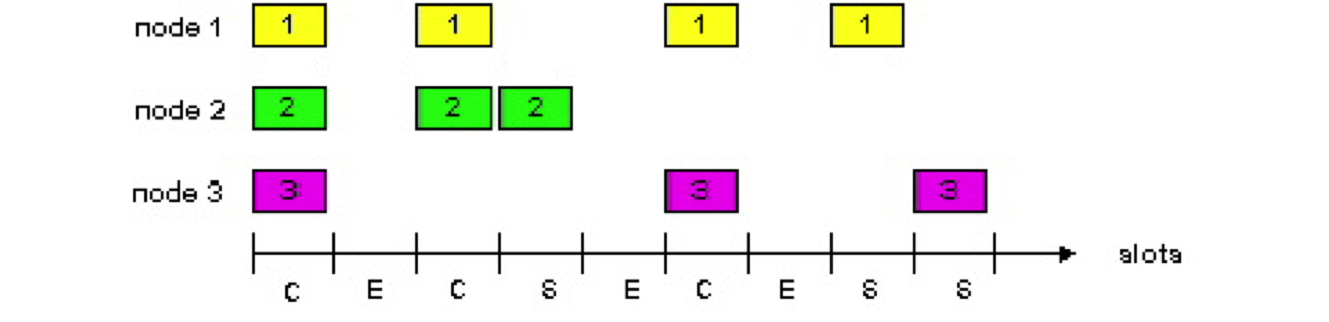
\includegraphics[width=8cm]{figs/06-aloha-part.png}
  \end{center}

\end{frame}
%---------------------------------------------------------------------
\begin{frame}
  \frametitle{ALOHA Particionado}
  Eficiencia
  \begin{itemize}
    \item $N$ nodos con {\em frames} a enviar. Probabilidad de enviar $p$.
    \item Probabilidad que un nodo dado pueda transmitir: $p(1-p)^{N-1}$
    \item Probabilidad que cualquier nodo pueda transmitir: $Np(1-p)^{N-1}$
    \item Maximo valor para esta expresión $\sim 0.368$
    \item Canal es utilizado a los más el $37\%$ del tiempo
  \end{itemize}

\end{frame}
%---------------------------------------------------------------------
\begin{frame}
  \frametitle{ALOHA}
  No hay sincronización al momento de empezar a transmitir
  \begin{itemize}
    \item Mayor probabilidad de colisiones
    \item Frame enviado en instante $t_0$ puede colisionar con frames enviados entre $[t_0-1,t_0+1]$
    \item Eficiencia $\sim 0.18$
  \end{itemize}

  \begin{center}
    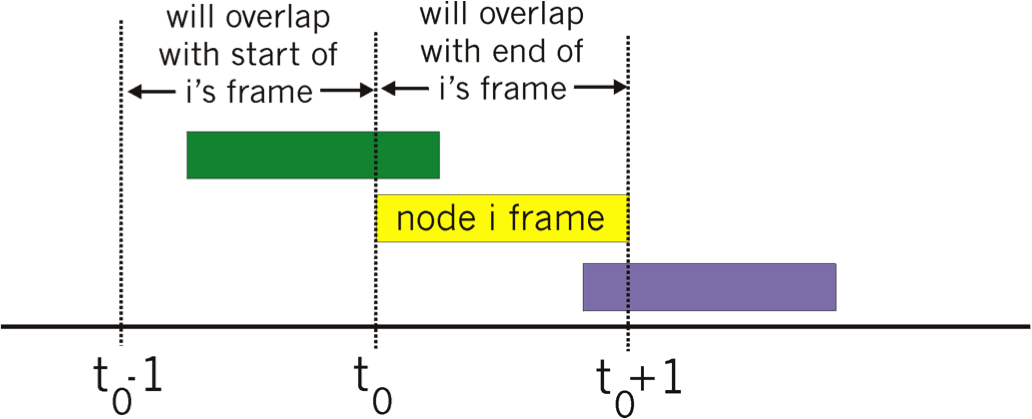
\includegraphics[width=8cm]{figs/06-aloha.png}
  \end{center}

\end{frame}

%---------------------------------------------------------------------
\begin{frame}
  \frametitle{CSMA}
  \framesubtitle{Carrier Sense Multiple Access}
  
  La idea es no interrumpir a los demás
  \begin{itemize}
    \item Emisor escucha antes de transmitir
    \item Si detecta canal inactivo, envía
    \item Si detecta canal activo, espera hasta dejar de detectar actividad
    \item Retrasos en la propagación permite que ocurran colisiones
  \end{itemize}

  \begin{center}
    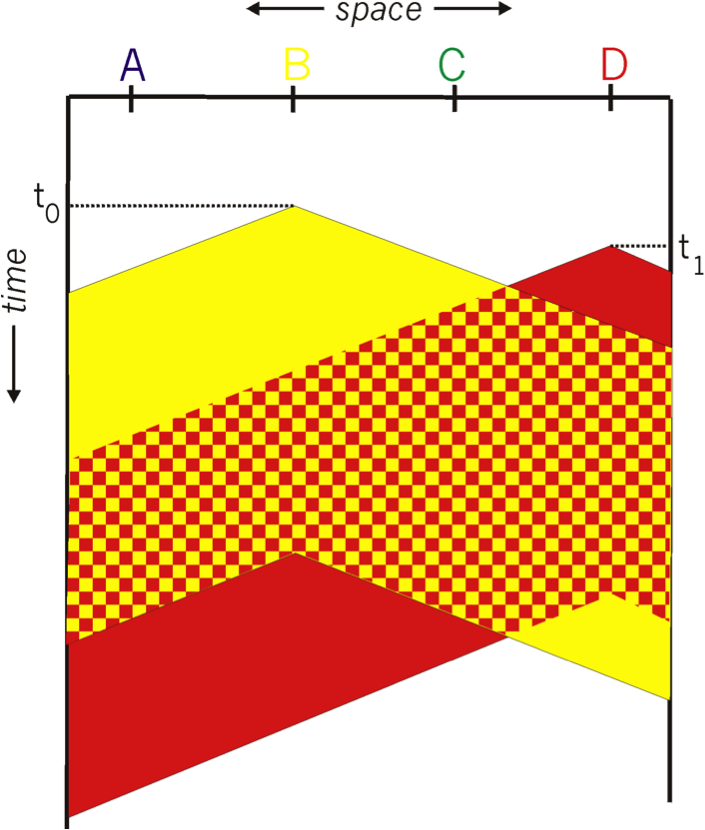
\includegraphics[width=4cm]{figs/06-csma.png}
  \end{center}


\end{frame}
%---------------------------------------------------------------------
\begin{frame}
  \frametitle{CSMA/CD}
  \framesubtitle{Carrier Sense Multiple Access / Colission Detection}

  \begin{itemize}
    \item Detección rápida de colisiones
    \item Transmisión se aborta en cuanto se detecta colisión, usando una {\em jam signal}
    \item Usando en LAN cableada (Ethernet): comparando nivel de fuerza de señales
    \item En WLAN: difícil de detectar
  \end{itemize}

  \begin{center}
    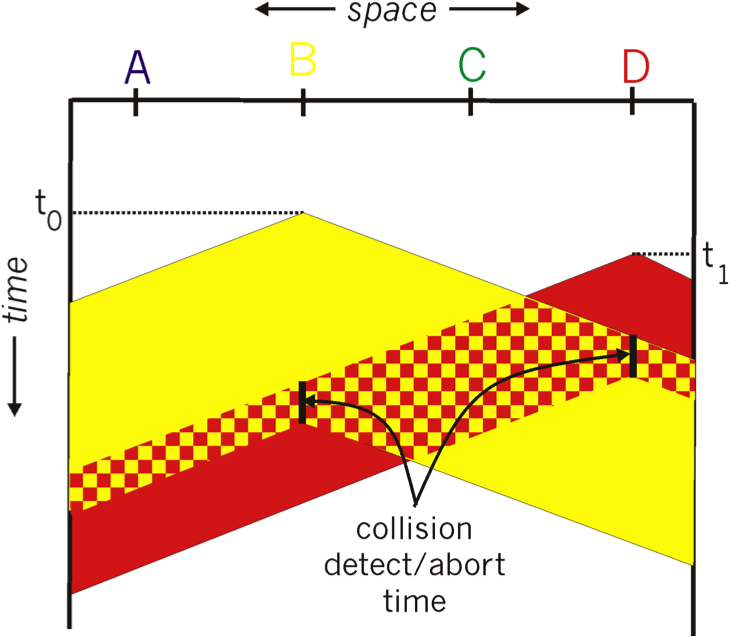
\includegraphics[width=4cm]{figs/06-csma-cd.png}
  \end{center}

\end{frame}

%%---------------------------------------------------------------------
\begin{frame}
  \frametitle{CSMA/CA}
  \framesubtitle{Carrier Sense Multiple Access / Colission Avoidance}

  \begin{itemize}
    \item Usado en WLAN.
    \item Si se detecta colisión se espera un tiempo aleatorio
    \item Complementado con paquetes adicionales:
      \begin{itemize}
        \item RTS (Request to Send)
        \item CTS (Clear to Send)
      \end{itemize}
  \end{itemize}

\end{frame}
%---------------------------------------------------------------------
\begin{frame}
  \frametitle{Protocolos por Turnos}
%  \framesubtitle{Carrier Sense Multiple Access / Colission Avoidance}

  \begin{itemize}
    \item Protocolos de particionamiento
      \begin{itemize}
        \item Eficientes con alta carga, canal desperdiciado con baja carga
      \end{itemize}
    \item Protocolos de acceso aleatorio
      \begin{itemize}
        \item Eficientes con baja carga, poco eficientes con alta carga
      \end{itemize}
  \end{itemize}
\end{frame}

%%---------------------------------------------------------------------
\begin{frame}
  \frametitle{Protocolos por Turnos}
  \framesubtitle{Master/Slave}
  
  Esquema master/slave
    \begin{itemize}
      \item Master invita a los slaves a transmitir
      \item Eficiente con terminales ``tontos''
      \item Alta latencia con muchos slaves
      \item Punto de falla centralizado
      \item Usado en Bluetooth
    \end{itemize}
  
  \begin{center}
    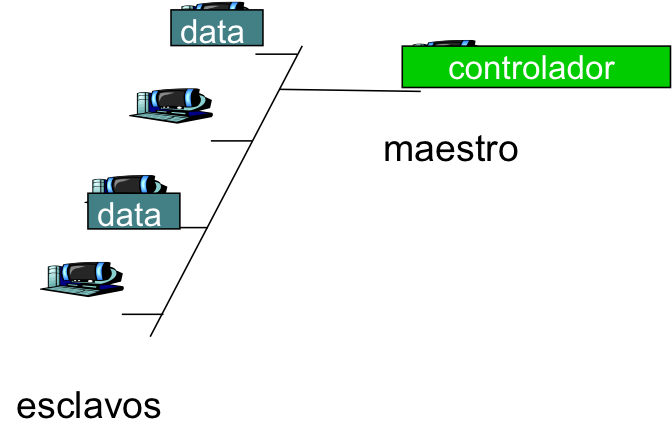
\includegraphics[width=4cm]{figs/06-turnos1.png}
  \end{center}

\end{frame}

%---------------------------------------------------------------------
\begin{frame}
  \frametitle{Protocolos por Turnos}
  \framesubtitle{Token}

  \begin{itemize}
    \item Nodos se pasan un {\em token}
    \item Sólo el que tiene el {\em token} puede transmitir
    \item Alta latencia con muchos miembros
    \item ¿Qué pasa si el nodo que tiene el {\em token} desaparece?
  \end{itemize}

  \begin{center}
    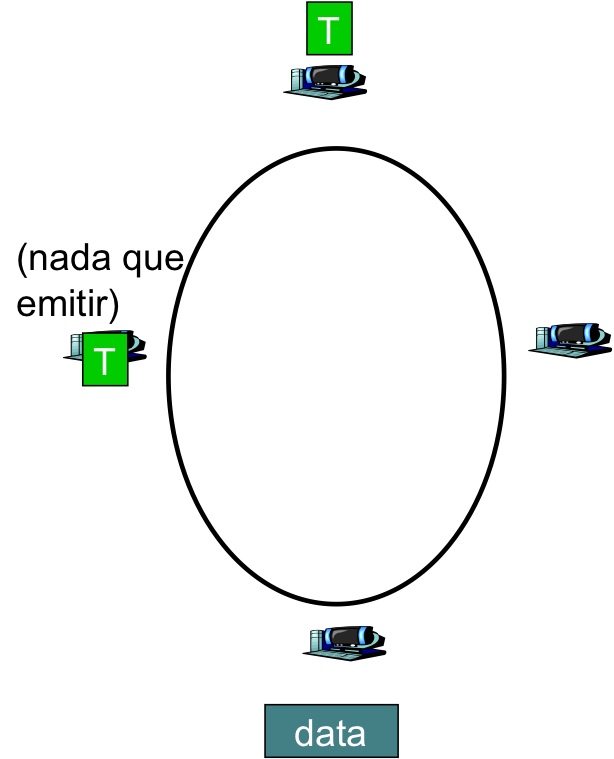
\includegraphics[width=4cm]{figs/06-turnos2.png}
  \end{center}

\end{frame}
%---------------------------------------------------------------------
\begin{frame}
  \frametitle{Direccionamiento en Capa de Enlace}

  \begin{itemize}
    \item Objetivo: asociar puertas de interfaz (NIC o switch) con destinos específicos
    \item {\em Dirección MAC}: 48-bit
      \begin{itemize}
        \item Dirección universal
        \item Particionadas por fabricante
        \item Guardada en ROM de NIC
        \item Puede ser enmascarada por software
      \end{itemize}
  \end{itemize}


\end{frame}
%---------------------------------------------------------------------
\begin{frame}
  \frametitle{Direccionamiento en Capa de Enlace}

  Dirección broadcast: FF-FF-FF-FF-FF-FF
  \begin{center}
    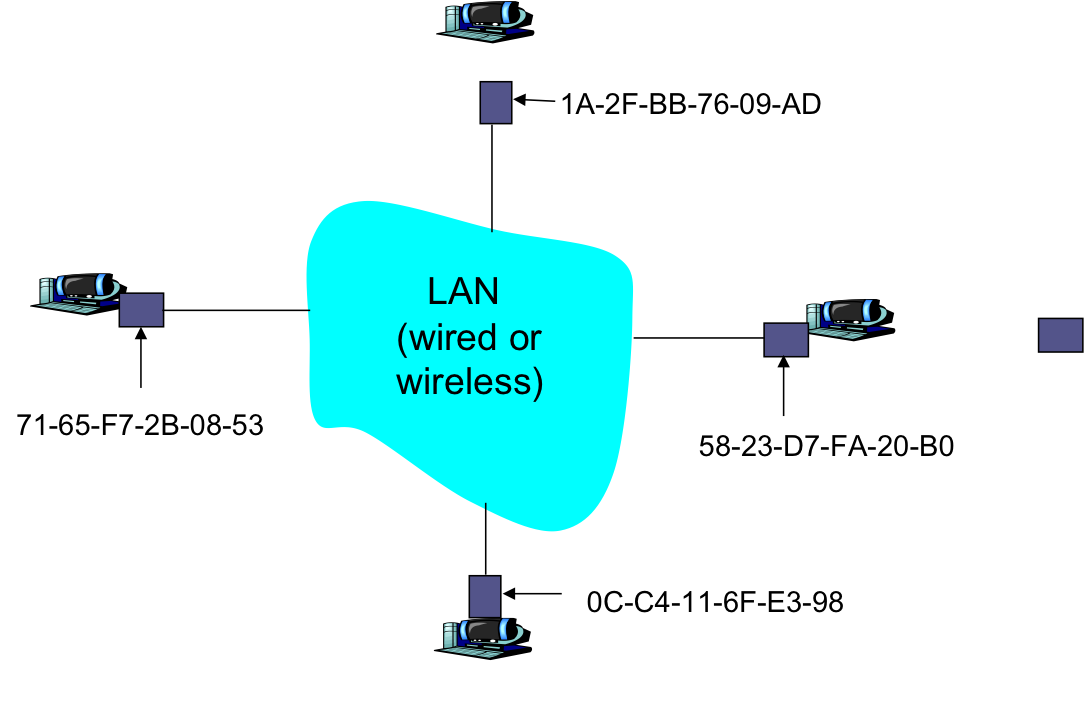
\includegraphics[width=6cm]{figs/06-lan-mac.png}
  \end{center}

\end{frame}
%---------------------------------------------------------------------
\begin{frame}
  \frametitle{Direccionamiento en Capa de Enlace}

  \begin{itemize}
    \item Direcciones asignadas por IEEE
    \item Cada fabricante compra un conjunto de direcciones
      \begin{itemize}
        \item 24-bit identifican al fabricante
        \item 24-bit identifican la tarjeta
      \end{itemize}
  \end{itemize}

\end{frame}
%---------------------------------------------------------------------
\begin{frame}
  \frametitle{Direccionamiento en Capa de Enlace}
  \framesubtitle{ARP: Address Resolution Protocol}
  
  \begin{itemize}
    \item Cada nodo (host,switch,router) mantiene una tabla ARP
    \item Tabla ARP contiene asociaciones $\langle \text{IP},\text{MAC},TTL \rangle$
    \item TTL: Time-To-Live, indica el tiempo que será recordada esa entrada
  \end{itemize}
  ¿Cómo determinar una dirección MAC?
  \begin{center}
    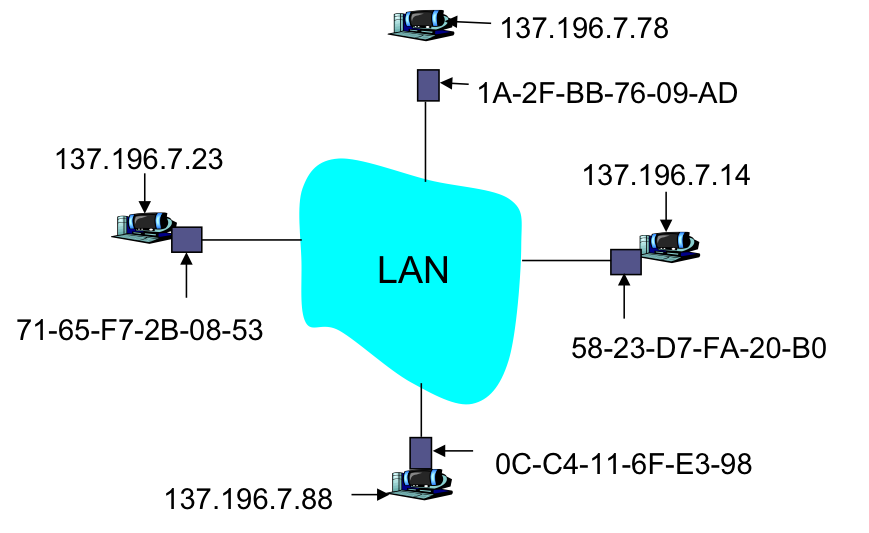
\includegraphics[width=6cm]{figs/06-arp.png}
  \end{center}
\end{frame}

%---------------------------------------------------------------------
\begin{frame}
  \frametitle{Direccionamiento en Capa de Enlace}
  \framesubtitle{ARP: Address Resolution Protocol}

  ¿Cómo determinar una dirección MAC?
  \begin{itemize}
    \item Si $A$ quiere comunicarse con $B$, que no está en su tabla
    \item $A$ envía mensaje ARP con IP de $B$ y broadcast FF-FF-FF-FF-FF-FF
    \item Todos reciben el mensaje
    \item Solo $B$ responde, con su dirección MAC
    \item $A$ guarda en su tabla ARP la asocación IP,MAC de $B$
  \end{itemize}

\end{frame}
%---------------------------------------------------------------------
\begin{frame}
  \frametitle{Direccionamiento en Capa de Enlace}
  \framesubtitle{Ruteo a distintas LAN}

  $A$ quiere enviar frame a $B$, vía $R$. $A$ conoce la IP de $B$
  \begin{itemize}
    \item $R$ mantiene dos tablas ARP, una para cada LAN
  \end{itemize}

  \begin{center}
    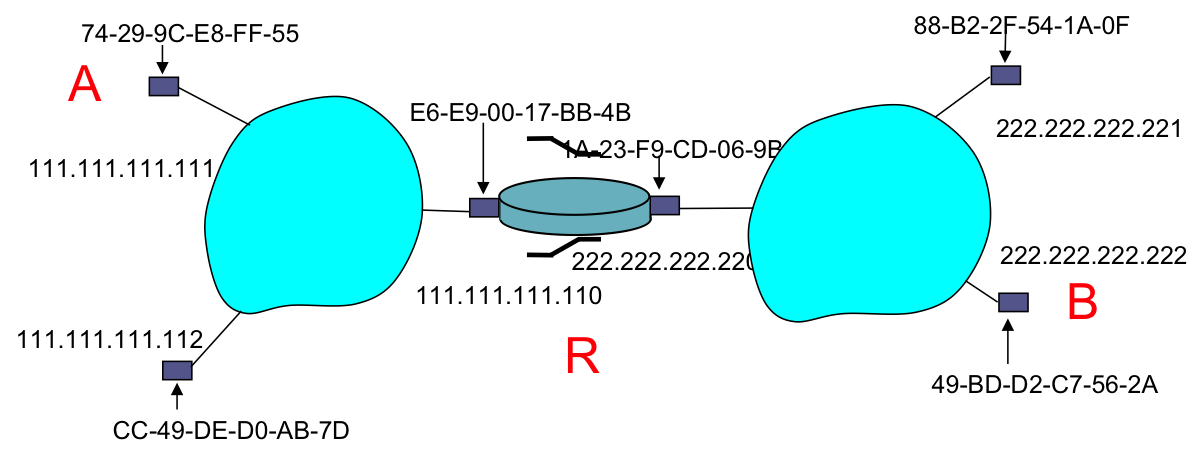
\includegraphics[width=9cm]{figs/06-arp-route.png}
  \end{center}

\end{frame}

%---------------------------------------------------------------------
\begin{frame}
  \frametitle{Hardware y Capa de Enlace}
  \framesubtitle{HUB}

  Dispositivo repetidor
  \begin{itemize}
    \item Cada {\em frame} que es recibido por una entrada es reenviado por {\em todas} las otras salidas
    \item Implementa topología de bus
    \item Todos los pares de nodos pueden tener colisiones
    \item NICs implementan CSMA/CD para detectar colisiones, pero el {\em hub} no  
  \end{itemize}

  \begin{center}
    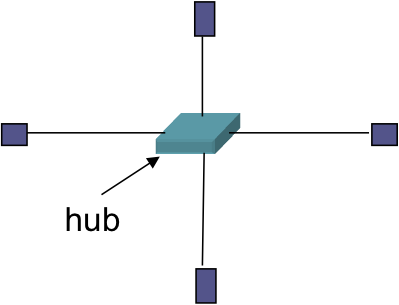
\includegraphics[width=4cm]{figs/06-hub.png}
  \end{center}


\end{frame}

%---------------------------------------------------------------------
\begin{frame}
  \frametitle{Hardware y Capa de Enlace}
  \framesubtitle{Switch}

  Dispositivo activo
  \begin{itemize}
    \item Almacena y reenvía {\em frames} Ethernet de manera selectiva
    \item Implementa CSMA/CD
    \item Transparente para nodos
    \item ¿Cómo se programan las entradas/salidas?
  \end{itemize}

  \begin{center}
    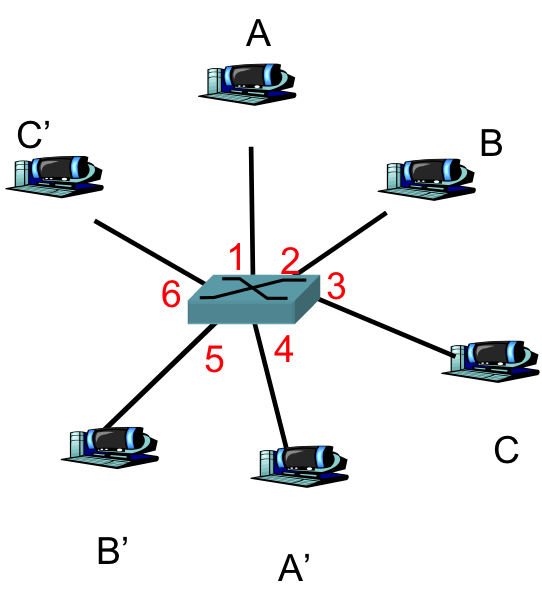
\includegraphics[width=4cm]{figs/06-switch.png}
  \end{center}


\end{frame}

%---------------------------------------------------------------------
\begin{frame}
  \frametitle{Hardware y Capa de Enlace}
  \framesubtitle{Switch}

  Aprendizaje de tablas
  \begin{itemize}
    \item {\em Switch} mantiene tablas de ubicación de nodos
    \item {\em Switch} aprende los nodos que están a su alcance
    \item Direcciones no conocidas se preguntan por {\em flooding}
  \end{itemize}

  \begin{center}
    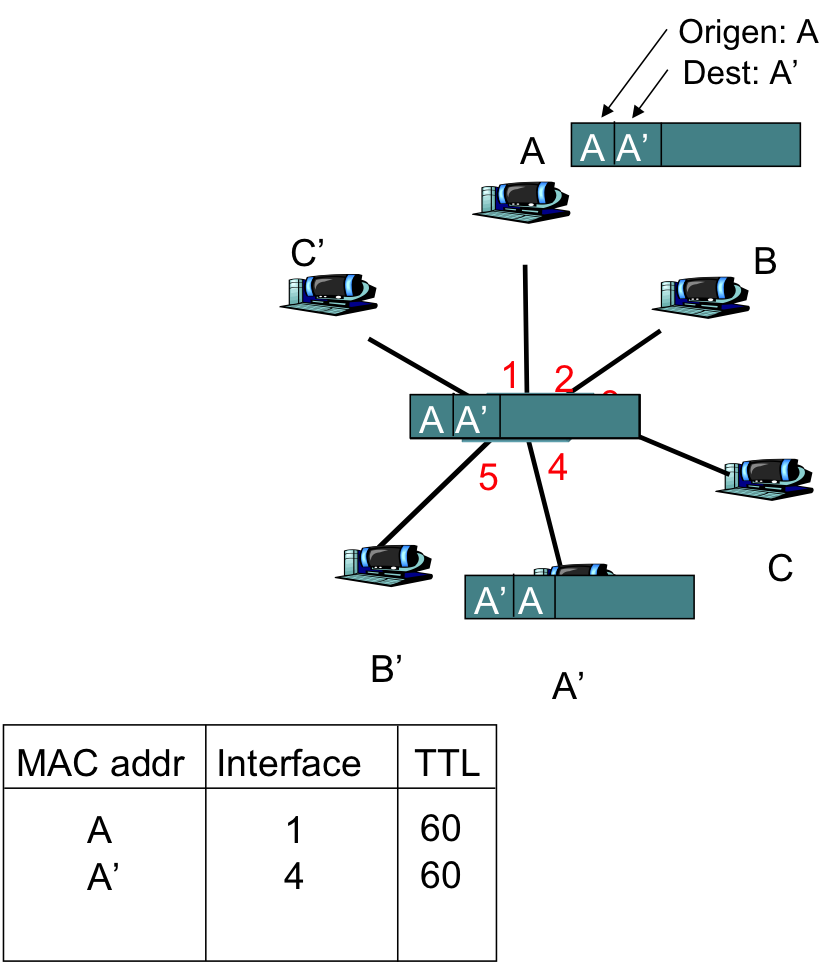
\includegraphics[width=4cm]{figs/06-switch-tablas.png}
  \end{center}

\end{frame}

%---------------------------------------------------------------------
\begin{frame}
  \frametitle{Hardware y Capa de Enlace}
  \framesubtitle{Switch: interconexiones}

  {\em Switches} pueden estar interconectados
  \begin{itemize}
    \item El método es el mismo
  \end{itemize}

  \begin{center}
    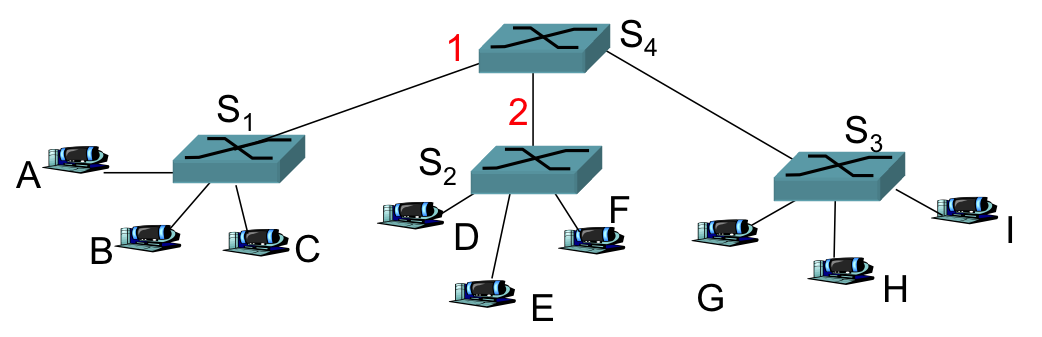
\includegraphics[width=8cm]{figs/06-switch-inter.png}
  \end{center}


\end{frame}

%---------------------------------------------------------------------
\begin{frame}
  \frametitle{Hardware y Capa de Enlace}
  \framesubtitle{Spanning Trees}

  ¿Cómo determinar el origen de B?
  
  \begin{center}
    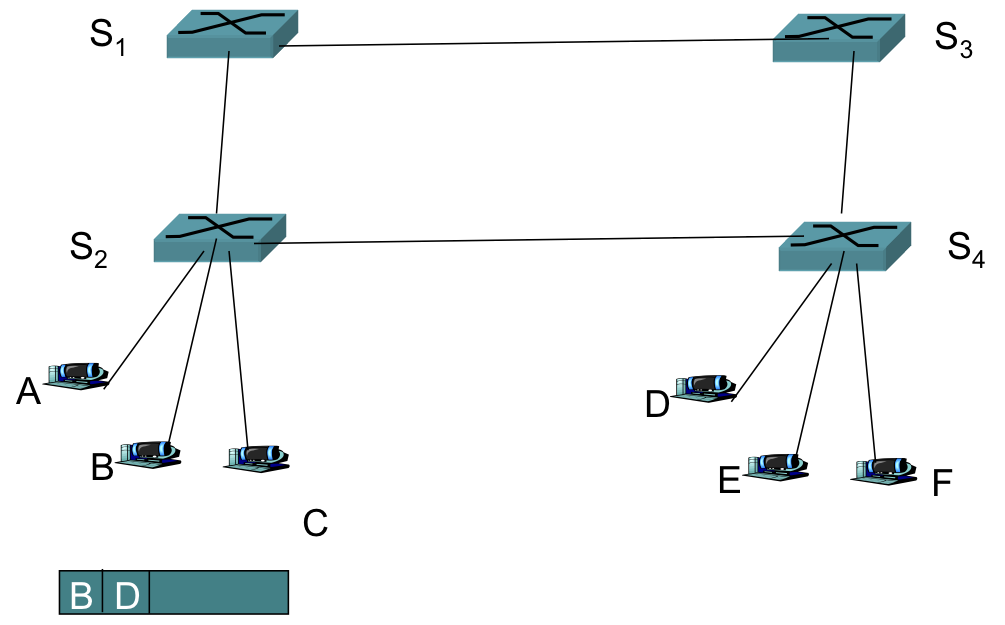
\includegraphics[width=8cm]{figs/06-switch-spanning.png}
  \end{center}

\end{frame}

%---------------------------------------------------------------------
\begin{frame}
  \frametitle{Hardware y Capa de Enlace}
  \framesubtitle{Spanning Tree Protocol}

  \begin{itemize}
    \item IEEE 802.1D
    \item Cada {\em switch} posee un identificador (único)
    \item Cada {\em switch} propaga su ID usando un {\em broadcast}:
      \begin{itemize}
        \item BPDU ({\em Bridge Protocol Data Unit}) frame
      \end{itemize}
    \item {\em Switches} con menor identificador pasan a ser raíz
    \item Caminos se eligen en dirección a la raíz
    \item ¿Minimum Spanning Tree?
  \end{itemize}

\end{frame}

%---------------------------------------------------------------------
\begin{frame}
  \frametitle{Hardware y Capa de Enlace}
  \framesubtitle{Spanning Tree Protocol}

  STP establece estados para los puertos
  \begin{itemize}
    \item {\bf Blocking}: no transmite {\em frames}. Sólo recibe BPDU
    \item {\bf Listening}: recibe y procesa BPDU. Puede pasar a {\em blocking} o {\em forwarding}
    \item {\bf Learning}: no transmite {\em frames}. Sólo procesa BPDU y actualiza tablas de transmisión
    \item {\bf Forwarding}: estado normal en que transmite {\em frames}
  \end{itemize}

\end{frame}  

%---------------------------------------------------------------------
\begin{frame}
  \frametitle{Control de Flujo}
%  \framesubtitle{Spanning Tree Protocol}

  \begin{itemize}
    \item Método para adaptar velocidad entre emisor y receptor
    \item {\em Switches} reciben datos desde diferentes interfaces
    \item Dos métodos basados en confirmación de receción
      \begin{itemize}
        \item Sliding Window
        \item Stop \& Wait
      \end{itemize}
  \end{itemize}

\end{frame}  

%---------------------------------------------------------------------
\begin{frame}
  \frametitle{Control de Flujo}
  \framesubtitle{Stop \& Wait}

  \begin{center}
    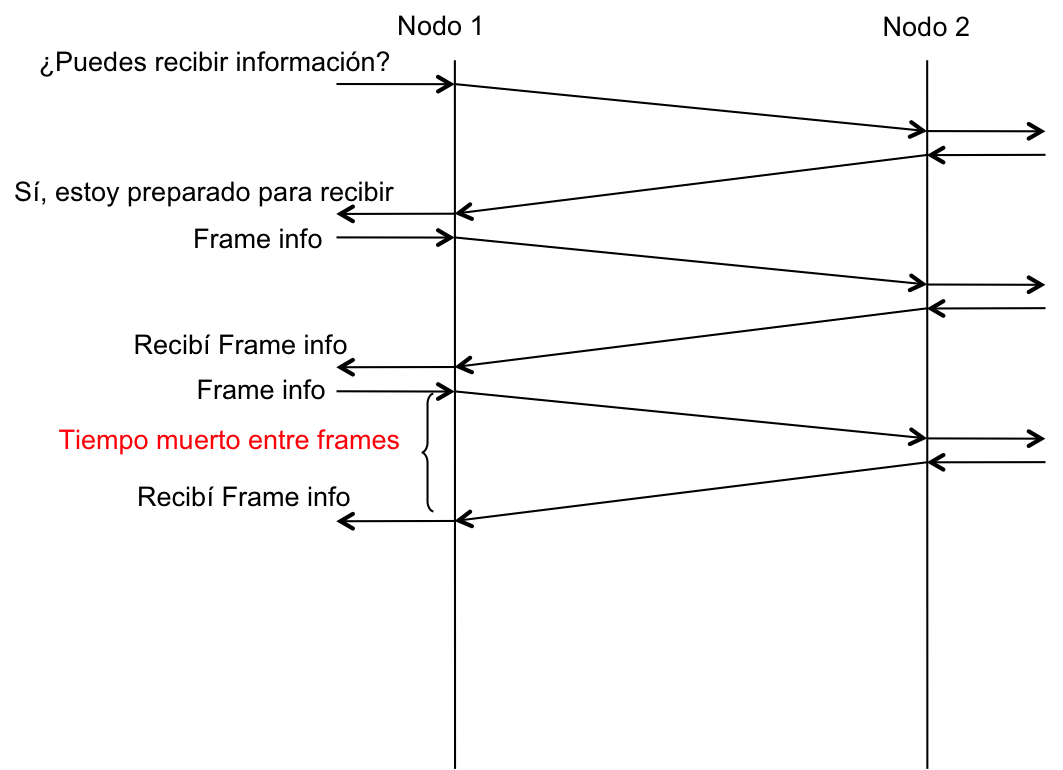
\includegraphics[width=10cm]{figs/06-flujo-stopwait.png}
  \end{center}


\end{frame}

%---------------------------------------------------------------------
\begin{frame}
  \frametitle{Control de Flujo}
  \framesubtitle{Sliding Window}

  \begin{center}
    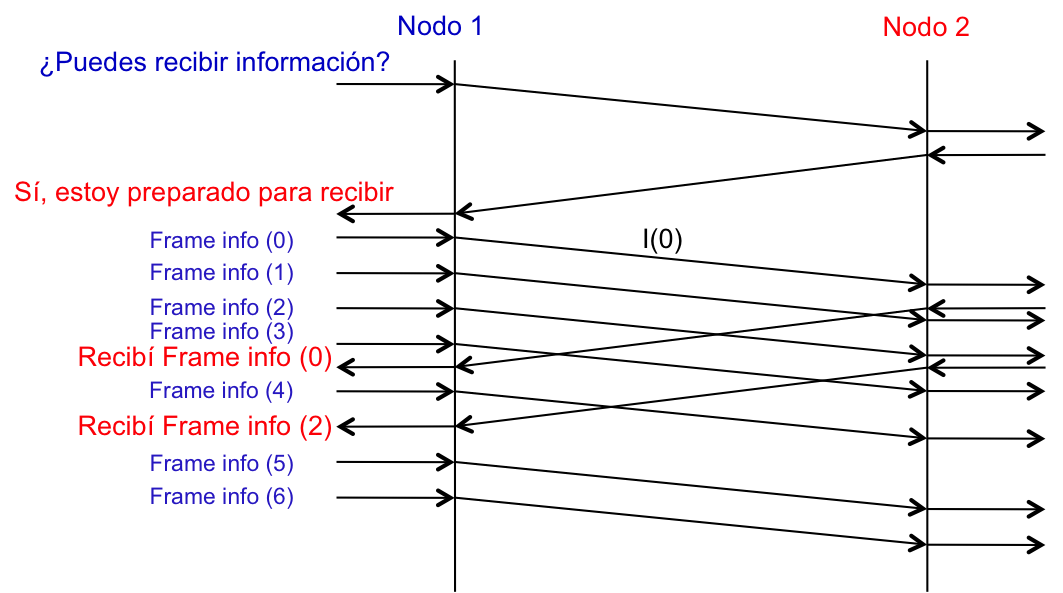
\includegraphics[width=10cm]{figs/06-flujo-sliding.png}
  \end{center}

\end{frame}


%---------------------------------------------------------------------
%---------------------------------------------------------------------
\end{document}